% arara: pdflatex
% arara: nomencl
% arara: pdflatex

%%%%%%%%%%%%%%%%%%%%%%%%%%%%%%%%%%%%%%%%%%%%%%%%%%%%%%%
%%      Para começar a usar este template, primeiro, %%
%% você dever criar uma conta no ShareLates. Depois, %%
%% vá nasopções no canto esquerdo superior da tela e %%
%% clique em "Copiar Projeto". Dê um novo nome para  %%
%% o projeto. This work has the LPPL maintenance     %%
%% status `maintained' The Currentt Maintainer of    %%
%% this work are:                                    %%
%%                                                   %%
%%        Ednardo Moreira Rodrigues (UFC/DEE)        %%
%%                      and                          %%
%%        Alan Batista de Oliveira (UFC/DEE)         %%
%%                                                   %%
%% Review:                                           %%
%%                                                   %%
%% - Eliene Maria Vieira de Moura;                   %%
%% - Francisco Edvander Pires Santos;                %%  
%% - Izabel Lima dos Santos;                         %%
%% - Juliana Soares Lima;                            %%
%% - Kalline Yasmin Soares Feitosa.                  %%
%%                                                   %%
%% This work may be distributed and/or modified under%%
%% theconditions of the LaTeX Project Public License,%%
%% either version 1.3 of this license or (at your    %%
%% option) any                                       %%
%% later version. The latest version of this license %%
%% is in http://www.latex-project.org/lppl.txt and   %%
%% version 1.3 or later is part of all distributions %%
%% of LaTeX version 2005/12/01 or later.             %%
%% The First Maintainer of this work was:            %%
%% Thiago Nascimento  (UECE)                         %%
%% Project available on:                             %%
%% https://github.com/thiagodnf/uecetex2             %%
%% Further information about abnTeX2                 %%
%% are available on http://abntex2.googlecode.com/   %%
%%%%%%%%%%%%%%%%%%%%%%%%%%%%%%%%%%%%%%%%%%%%%%%%%%%%%%%

\documentclass[        
    a4paper,          % Tamanho da folha A4
    12pt,             % Tamanho da fonte 12pt
    chapter=TITLE,    % Todos os capitulos devem ter caixa alta
    section=Title,    % Todas as secoes devem ter caixa alta somente na primeira letra
    subsection=Title, % Todas as subsecoes devem ter caixa alta somente na primeira letra
    oneside,          % Usada para impressao em apenas uma face do papel
    english,          % Hifenizacoes em ingles
    spanish,          % Hifenizacoes em espanhol
    brazil,           % Ultimo idioma eh o idioma padrao do documento
    fleqn             % Coloca as equações alinhadas a esquerda
]{abntex2}

%%%%%%%%%%%%%%%%%%%%%%%%%%%%%%%%%%%%%%%%%%%%%%%%%%%%%%%
%%      Para começar a usar este template, primeiro, %%
%% você dever criar uma conta no ShareLates. Depois, %%
%% vá nasopções no canto esquerdo superior da tela e %%
%% clique em "Copiar Projeto". Dê um novo nome para  %%
%% o projeto. This work has the LPPL maintenance     %%
%% status `maintained' The Currentt Maintainer of    %%
%% this work are:                                    %%
%%                                                   %%
%%        Ednardo Moreira Rodrigues (UFC/DEE)        %%
%%                      and                          %%
%%        Alan Batista de Oliveira (UFC/DEE)         %%
%%                                                   %%
%% Review:                                           %%
%%                                                   %%
%% - Eliene Maria Vieira de Moura;                   %%
%% - Francisco Edvander Pires Santos;                %%  
%% - Izabel Lima dos Santos;                         %%
%% - Juliana Soares Lima;                            %%
%% - Kalline Yasmin Soares Feitosa.                  %%
%%                                                   %%
%% This work may be distributed and/or modified under%%
%% theconditions of the LaTeX Project Public License,%%
%% either version 1.3 of this license or (at your    %%
%% option) any                                       %%
%% later version. The latest version of this license %%
%% is in http://www.latex-project.org/lppl.txt and   %%
%% version 1.3 or later is part of all distributions %%
%% of LaTeX version 2005/12/01 or later.             %%
%% The First Maintainer of this work was:            %%
%% Thiago Nascimento  (UECE)                         %%
%% Project available on:                             %%
%% https://github.com/thiagodnf/uecetex2             %%
%% Further information about abnTeX2                 %%
%% are available on http://abntex2.googlecode.com/   %%
%%%%%%%%%%%%%%%%%%%%%%%%%%%%%%%%%%%%%%%%%%%%%%%%%%%%%%%

% \documentclass[        
%     a4paper,          % Tamanho da folha A4
%     12pt,             % Tamanho da fonte 12pt
%     chapter=TITLE,    % Todos os capitulos devem ter caixa alta
%     section=TITLE,    % Todas as secoes devem ter caixa alta
%     oneside,          % Usada para impressao em apenas uma face do papel
%     english,          % Hifenizacoes em ingles
%     spanish,          % Hifenizacoes em espanhol
%     brazil            % Ultimo idioma eh o idioma padrao do documento
% ]{abntex2}

% Importações de pacotes
% possibilita ctrl+c com acentos em português
\usepackage[utf8]{inputenc}                         % Acentuação direta
\usepackage[T1]{fontenc}                            % Codificação da fonte em 8 bits
\usepackage{graphicx}                               % Inserir figuras
\usepackage{amsfonts, amssymb, amsmath}             % Fonte e símbolos matemáticos
\usepackage{booktabs}                               % Comandos para tabelas
\usepackage{verbatim}                               % Texto é interpretado como escrito no documento
\usepackage{multirow, array}                        % Múltiplas linhas e colunas em tabelas
\usepackage{indentfirst}                            % Endenta o primeiro parágrafo de cada seção.
\usepackage{listings}                               % Utilizar codigo fonte no documento
\usepackage{xcolor}
\usepackage{microtype}                              % Para melhorias de justificação?
\usepackage[portuguese,ruled,lined]{algorithm2e}    % Escrever algoritmos
\usepackage{algorithmic}                            % Criar Algoritmos  
%\usepackage{float}                                 % Utilizado para criação de floats
\usepackage{amsgen}
\usepackage{lipsum}                                 % Usar a simulação de texto Lorem Ipsum
%\usepackage{titlesec}                              % Permite alterar os títulos do documento
\usepackage{tocloft}                                % Permite alterar a formatação do Sumário
\usepackage{etoolbox}                               % Usado para alterar a fonte da Section no Sumário
\usepackage[acronym,nogroupskip,nonumberlist]{glossaries}   % Permite fazer o glossario
\usepackage[font=singlespacing]{caption}                                % Altera o comportamento da tag caption
\usepackage[alf, abnt-emphasize=bf, recuo=0cm, abnt-etal-cite=2, abnt-etal-list=0, abnt-etal-text=it]{abntex2cite}  % Citações padrão ABNT
%\usepackage[bottom]{footmisc}                      % Mantém as notas de rodapé sempre na mesma posição
%\usepackage{times}                                 % Usa a fonte Times
\usepackage{mathptmx}                               % Usa a fonte Times New Roman										
%\usepackage{lmodern}                               % Usa a fonte Latin Modern
%\usepackage{subfig}                                % Posicionamento de figuras
%\usepackage{scalefnt}                              % Permite redimensionar tamanho da fonte
%\usepackage{color, colortbl}                       % Comandos de cores
%\usepackage{lscape}                                % Permite páginas em modo "paisagem"
\usepackage{ae, aecompl}                            % Fontes de alta qualidade
%\usepackage{picinpar}                              % Dispor imagens em parágrafos
\usepackage{latexsym}                               % Símbolos matemáticos
%\usepackage{upgreek}                               % Fonte letras gregas
\usepackage{appendix}                               % Gerar o apendice no final do documento
\usepackage{paracol}                                % Criar paragrafos sem identacao
\usepackage{lib/ufctex}		                        % Biblioteca com as normas da UFC para trabalhos academicos
\usepackage{pdfpages}                               % Incluir pdf no documento
\usepackage{amsmath}                                % Usar equacoes matematicas


% Meus Pacotes - Não pertencem ao template original
% adicionar os simbolos dos question\'arios
\usepackage{threeparttable}
\usepackage{wasysym}
\usepackage{float}

% Organiza e gera a lista de abreviaturas, simbolos e glossario
\makeglossaries

% Gera o Indice do documento
\makeindex


%%%%%%%%%%%%%%%%%%%%%%%%%%%%%%%%%%%%%%%%%%%%%%%%%%%%%
%%          Configuracoes do ufctex                %%
%%%%%%%%%%%%%%%%%%%%%%%%%%%%%%%%%%%%%%%%%%%%%%%%%%%%%

% Opcoes disponiveis

\trabalhoacademico{tccgraduacao}
%\trabalhoacademico{tccespecializacao}
%\trabalhoacademico{dissertacao}
%\trabalhoacademico{tese}

% Define se o trabalho eh uma qualificacao
% Coloque 'nao' para versao final do trabalho

\ehqualificacao{nao}

% Remove as bordas vermelhas e verdes do PDF gerado
% Coloque 'sim' pare remover

\removerbordasdohyperlink{sim} 

% Adiciona a cor Azul a todos os hyperlinks

\cordohyperlink{nao}

%%%%%%%%%%%%%%%%%%%%%%%%%%%%%%%%%%%%%%%%%%%%%%%%%%%%%
%%          Informação sobre a IES                 %%
%%%%%%%%%%%%%%%%%%%%%%%%%%%%%%%%%%%%%%%%%%%%%%%%%%%%%

\ies{Universidade Federal do Ceará}
\iessigla{UFC}
\centro{Campus Quixadá}

%%%%%%%%%%%%%%%%%%%%%%%%%%%%%%%%%%%%%%%%%%%%%%%%%%%%%
%%        Informação para TCC de Graduacao %%
%%%%%%%%%%%%%%%%%%%%%%%%%%%%%%%%%%%%%%%%%%%%%%%%%%%%%

\graduacaoem{Sistemas de Informação}
\habilitacao{bacharel} % Pode colocar tambem 'licenciada'

%%%%%%%%%%%%%%%%%%%%%%%%%%%%%%%%%%%%%%%%%%%%%%%%%%%%%
%%     Informação para TCC de Especializacao       %%
%%%%%%%%%%%%%%%%%%%%%%%%%%%%%%%%%%%%%%%%%%%%%%%%%%%%%

% \especializacaoem{Descargas Atmosféricas}

%%%%%%%%%%%%%%%%%%%%%%%%%%%%%%%%%%%%%%%%%%%%%%%%%%%%%
%%         Informação para Dissertacao             %%
%%%%%%%%%%%%%%%%%%%%%%%%%%%%%%%%%%%%%%%%%%%%%%%%%%%%%

% \programamestrado{Programa de Pós-Graduação em Xxxxxxx}
% \nomedomestrado{Mestrado Acadêmico em Xxxxxxx}
% \mestreem{Engenharia Xxxxxx}
% \areadeconcentracaomestrado{Engenharia Xxxxxx}

%%%%%%%%%%%%%%%%%%%%%%%%%%%%%%%%%%%%%%%%%%%%%%%%%%%%%
%%               Informação para Tese              %%
%%%%%%%%%%%%%%%%%%%%%%%%%%%%%%%%%%%%%%%%%%%%%%%%%%%%%

% \programadoutorado{Programa de Pós-Graduação em Xxxxxx}
% \nomedodoutorado{Doutorado em Xxxxxxx}
% \doutorem{Engenharia Xxxxxx}
% \areadeconcentracaodoutorado{Engenharia Xxxxxxx}

%%%%%%%%%%%%%%%%%%%%%%%%%%%%%%%%%%%%%%%%%%%%%%
%%  Informacoes relacionadas ao trabalho     %%
%%%%%%%%%%%%%%%%%%%%%%%%%%%%%%%%%%%%%%%%%%%%%%

\autor{Marciano Machado Saraiva}
\titulo{Ambiente Virtual de Aprendizagem para Auxiliar no Processo de Ensino e Aprendizagem de Matemática}
\data{2016}
\local{Quixadá}

% Exemplo: \dataaprovacao{01 de Janeiro de 2012}
\dataaprovacao{}

%%%%%%%%%%%%%%%%%%%%%%%%%%%%%%%%%%%%%%%%%%%%%
%%     Informação sobre o Orientador       %%
%%%%%%%%%%%%%%%%%%%%%%%%%%%%%%%%%%%%%%%%%%%%%

\orientador{Prof. Me. Samy Soares Passos de Sá}
\orientadories{Universidade Federal do Ceará (UFC)}
\orientadorcentro{Campus Quixadá}
\orientadorfeminino{nao} % Coloque 'sim' se for do sexo feminino

%%%%%%%%%%%%%%%%%%%%%%%%%%%%%%%%%%%%%%%%%%%%%
%%      Informação sobre o Co-orientador   %%
%%%%%%%%%%%%%%%%%%%%%%%%%%%%%%%%%%%%%%%%%%%%%

% Deixe o nome do coorientador em branco para remover do documento

\coorientador{}
\coorientadories{Universidade Co-orientador (SIGLA)}
\coorientadorcentro{Centro do Co-orientador (SIGLA)}
\coorientadorfeminino{nao} % Coloque 'sim' se for do sexo feminino

%%%%%%%%%%%%%%%%%%%%%%%%%%%%%%%%%%%%%%%%%%%%%
%%      Informação sobre a banca           %%
%%%%%%%%%%%%%%%%%%%%%%%%%%%%%%%%%%%%%%%%%%%%%

% Atenção! Deixe o nome do membro da banca para remover da folha de aprovacao

% Exemplo de uso:
% \membrodabancadois{Prof. Dr. Fulano de Tal}
% \membrodabancadoisies{Universidade Federal do Ceará - UFC}

\membrodabancadois{Prof. Dr. Wladmir Araujo Tavares}
\membrodabancadoiscentro{Campus Quixadá}
\membrodabancadoisies{Universidade Federal do Ceará - UFC}

\membrodabancatres{Prof. Me. Carlos Roberto Rodrigues Filho}
\membrodabancatrescentro{Campus Quixadá}
\membrodabancatresies{Universidade Federal do Ceará - UFC}

% \membrodabancaquatro{}
% \membrodabancaquatrocentro{Centro de Ciências e Tecnologia (CCT)}
% \membrodabancaquatroies{Universidade do Membro da Banca Quatro (SIGLA)}
% \membrodabancacinco{}
% \membrodabancacincocentro{Teste}
% \membrodabancacincoies{Universidade do Membro da Banca Cinco (SIGLA)}
% \membrodabancaseis{}
% \membrodabancaseiscentro{}
% \membrodabancaseisies{Universidade do Membro da Banca Seis (SIGLA)}

\begin{document}	

	% Elementos pré-textuais
	\imprimircapa
	\imprimirfolhaderosto{}
	\imprimirfichacatalografica{elementos-pre-textuais/ficha-catalografica}
	%\imprimirerrata{elementos-pre-textuais/errata}
	\imprimirfolhadeaprovacao
	\imprimirdedicatoria{elementos-pre-textuais/dedicatoria}
	\imprimiragradecimentos{elementos-pre-textuais/agradecimentos}
	\imprimirepigrafe{elementos-pre-textuais/epigrafe}
	\imprimirresumo{elementos-pre-textuais/resumo}
	\imprimirabstract{elementos-pre-textuais/abstract}
	\imprimirlistadeilustracoes
	\imprimirlistadetabelas
	%\imprimirlistadequadros
	%\imprimirlistadealgoritmos
	%\imprimirlistadecodigosfonte
 	\imprimirlistadeabreviaturasesiglas
	\imprimirlistadesimbolos{elementos-pre-textuais/lista-de-simbolos}   
	\imprimirsumario
	
	%Elementos textuais
	\textual
	\chapter{INTRODUÇÃO}
\label{cap:introducao}

A Matemática, como ciência, tem uma relação muito especial com as novas tecnologias desde as calculadoras aos computadores, sistemas 
multim\'idia, e a \textit{Internet}. No entanto, alguns professores costumam demorar a perceber como tirar proveito destas tecnologias como 
ferramentas de trabalho \cite{da1997ensino}. \`A medida que a quantidade de recursos tecnológicos na sala de aula foram aumentando, 
tornou-se conveniente a criação de novas metodologias de ensino, especificamente na Educação Matemática. A busca por novas 
metodologias de ensino que fazem uso destes recursos procura fazer da matemática uma disciplina atraente e desvinculada do ensino 
tradicional, que já se mostrou ineficiente \cite{silva2009ambiente}.

Grande parte dos alunos, em todas as faixas etárias, tem dificuldades em aprender matemática, e muitas vezes essas dificuldades ocorrem 
não pela falta de atenção ou por não gostar do conteúdo, mas por fatores mentais, psicológicos e pedag\'ogicos que envolvem uma série de 
trabalhos e conceitos que 
precisam ser desenvolvidos \cite{de2006dificuldades}. Mas como auxiliar alunos com dificuldades na aprendizagem da matemática? Em busca 
dessa resposta, diferentes sistemas de \textit{software} foram desenvolvidos buscando servir \`a  educação Matem\'atica. Em 2006, Salman 
Khan fundou a Khan Academy, uma organização educacional que tem por objetivo oferecer exercícios, vídeos de instrução e um painel de 
aprendizado personalizado que habilita os estudantes a aprender no seu próprio ritmo dentro e fora da sala de aula \cite{khan2012one}. A 
plataforma criada por Khan utiliza vídeo-aulas e resolução de problemas para ensinar seus alunos, permitindo que cada um aprenda de forma 
independente e no seu pr\'oprio ritmo. Uma outra plataforma também  importante nessa área, \'e o ActiveMath 
\cite{melis2001activemath}, uma plataforma que permite aos estudantes desfrutarem da experiência de estudar num 
curso gerado dinamicamente. Nessa plataforma, os conte\'udos s\~ao representados no formato XML \cite{bray1998extensible} e armazenados 
numa base de conhecimento\footnote{São bases de dados ou conhecimentos acumulados sobre um determinado assunto.}, onde s\~ao recuperados para gerar cursos individuais de acordo com regras 
pedagógicas\footnote{S\~ao regras que determinam quando e quais ferramentas do sistema devem ser apresentadas e em que ordem.} 
\cite{melis2004activemath}. Estes e outros trabalhos serão apresentados com mais detalhes na \autoref{cap:trabalhos-relacionados}.

O presente trabalho apresenta o projeto de um \gls{ava} \cite{valentini2010aprendizagem}, para auxiliar 
estudantes no ensino e aprendizagem de conteúdos matemáticos. Este ambiente se propõe a servir como ferramenta para estudantes que buscam 
estudar fora do ambiente escolar e em seu próprio ritmo. O ambiente também dará suporte ao ensino e aprendizagem em sala de aula, 
auxiliando professores com informações relevantes sobre o andamento do aprendizado de cada um de seus alunos, além das dificuldades que os 
mesmos apresentam.

A ideia deste AVA surgiu quando professores das disciplinas de matemática da Universidade Federal do Cear\'a observaram um grande número de 
reprovações e desistências em suas turmas. Segundo os professores, um dos fatores que pode ser o causador são as deficiências de formação em 
matemática desde o ensino médio, e, por isso, faltaria aos alunos a base para compreender os novos assuntos. Essa suspeita é reforçada por 
um estudo realizado pela Organização para a Cooperação e Desenvolvimento Econômico \cite{pisainfocus2016}. Esse estudo revelou que 67.1\% 
dos alunos brasileiros ainda estavam abaixo do nível 2 (os níveis são de 1 a 6) de proficiência em matem\'atica, deixando o país em 58º 
lugar 
na escala do PISA\footnote{O 
Programa Internacional de Avaliação de Estudantes (Pisa) é uma iniciativa de avaliação comparada, aplicada a estudantes na faixa dos 15 
anos, idade em que se pressupõe o término da escolaridade básica obrigatória na maioria dos países e que visa melhorar as políticas e 
resultados educacionais.}, ficando na frente apenas de países como Jordânia, Catar, Colômbia, Peru e Indonésia na \'ultima posi\c{c}\~ao. 
Sendo que somente 0,8\% dos estudantes brasileiros alcançaram os últimos patamares.

\section{Objetivos do Trabalho}

Este trabalho objetiva apresentar o projeto de um AVA para auxiliar no processo de ensino e aprendizagem de matemática por alunos dentro e 
fora da sala de aula, buscando contribuir com o processo de ensino e aprendizagem de matem\'atica. 

Como objetivos específicos para este trabalho, temos: 
[DEIXA PRA FAZER COM O SAMY]
\begin{alineas}
  \item Levantar os requisitos do sistema.
  \item Desenvolver os módulos com funções de administração do sistema.
  \item Desenvolver os módulos com funções que serão utilizadas pelos estudantes aplicando técnicas de Gamificação.
  \item Avaliar a interface do ambiente desenvolvido aplicando um teste de usabilidade com estudantes do ensino m\'edio e universit\'arios.
\end{alineas}


\section{Divisão do Trabalho}

Fundamentando-se na problemática mencionada e tendo em vista o objeto de estudo, dividimos esta monografia em quatro capítulos. No 
segundo cap\'itulo, destacaremos os aspectos teóricos sobre ensino e aprendizagem, assim como as tradicionais metodologias de ensino e as 
apoiadas por computador. Abordaremos tamb\'em conceitos de gamificação e os trabalhos que servem de refer\^encia para os conceitos e 
id\'eias utilizadas no trabalho aqui desenvolvido. No terceiro capítulo, discutiremos a concepção, construção e modelagem do sistema, 
apresentando o que o mesmo deve possuir e por que, e no quarto capítulo, apresentaremos os resultados alcan\c{c}ados.
	\chapter{REVISÃO BIBLIOGRÁFICA}
\label{cap:fundamentacao-teorica}

Este capítulo aborda os seguintes temas: metodologias no ensino da matemática, conceito de ambientes virtuais de aprendizagem, o uso da gamificação aplicada em AVAs, e, por fim, o que está sendo 
desenvolvido por outros pesquisadores da área.

\section{Metodologias no Ensino da Matemática}

Ao longo da história, várias metodologias e abordagens matemáticas foram utilizadas visando a melhoria do ensino. Segundo \citeonline{hammes2003tendencias}, algumas delas foram aula expositiva, 
resolução de problemas, modelagem matemática, e o uso de computadores. Nas seções a seguir, descreveremos cada uma delas.

\subsection{Aula expositiva}

Em uma aula expositiva, o professor comumente faz uma revisão da aula anterior, apresenta o novo conteúdo e passa aos alunos uma série de exercícios de fixação. Esse novo conteúdo é apresentado de 
forma oral ou escrita, sem levar em consideração o conhecimento prévio dos estudantes nem tempo para perguntas. Essa é, sem dúvida, uma das mais utilizadas e antigas metodologias existentes. Durante 
o século passado, aulas expositivas foram o único processo empregado em sala de aula pelos professores. Dessa forma, a aula expositiva pode ser considerada cansativa e desinteressante, já que o aluno não participa do processo de ensino  \cite{hammes2003tendencias}. Para \citeonline{de1996gerencia}, essa abordagem possui diversos problemas. \citeonline{de1996gerencia} sugere que a escola tradicional não somente está desatualizada para atender às necessidades 
crescentes da sociedade contemporânea, como também apresenta algumas características que inibem o desenvolvimento do potencial de criação dos alunos:

\begin{alineascomponto}
\item Destaca-se a incompetência, a ignorância e a incapacidade do aluno, deixando de assinalar os talentos e habilidades de cada um; 
\item O ensino voltado para o passado, em que se enfatiza a reprodução e a memorização do conhecimento;
\item Desconsidera-se a imaginação e a fantasia como dimensões importantes da mente;
\item Exercício de resposta única, em que se cultua o medo do erro e do fracasso;
\item A obediência, dependência, passividade e conformismo são os traços mais cultivados;
\item Descaso em cultivar uma visão otimista do futuro;
\item As habilidades cognitivas são desenvolvidas de forma limitada;
\end{alineascomponto}

Autores como \citeonline{lopes1995aula}, defendem que a aula expositiva ``poderá ser transformada em uma atividade dinâmica, participativa e estimuladora do pensamento critico do aluno''. Uma alternativa descrita por \citeonline{lopes1995aula} é transformar a aula expositiva em uma aula expositiva dialógica. Essa forma de aula expositiva utiliza o diálogo entre professor e aluno para estabelecer uma relação de intercambio de conhecimentos e experiências \cite{lopes1995aula}. De acordo com \citeonline{freire1982educaccao}, o ensino dialógico se contrapõe ao ensino 
autoritário,  transformando  a  sala  de  aula  em  ambiente  propicio  à  reelaboração  e produção de conhecimentos.


\subsection{Resolução de problemas}\label{resolucao_problemas}

A resolução de problemas deve ser entendida como uma oportunidade para o aluno obter novos conhecimentos e não apenas conhecimentos prontos que fazem parte da nossa história. Ela ajuda o aluno a desenvolver sua autonomia buscando as respostas para seus próprios questionamentos. \citeonline{fossa1998tendencias} ressaltam  que esta metodologia visa o desenvolvimento de habilidades metacognitivas, favorecendo a reflexão e o questionamento do aluno que aprende a pensar por si mesmo, levantando hipóteses, testando-as, tirando conclusões e até discutindo-as com os colegas.

Na metodologia de resolução de problemas, é importante que os problemas apresentem uma incógnita que necessite ser descoberta. Para resolvê-los, o aluno terá que inventar estratégias e gerar novas ideias. Segundo \citeonline{dante1991didatica} é importante que o problema possa gerar muitos processos de pensamento, levantar muitas hipóteses e propiciar várias estratégias de solução. O pensar e o fazer criativo devem ser componentes fundamentais no processo de resolução de problemas.

\subsection{Modelagem Matemática}

De acordo com \citeonline[p.~16]{bassanezi2002ensino}, “[...] a modelagem consiste na arte de transformar situações da realidade em problemas matemáticos cujas soluções devem ser interpretadas na linguagem do mundo real”. Nas metodologias anteriores, o processo de ensino é deflagrado pelo professor. Na Modelagem Matemática, o processo é compartilhado com o grupo de alunos, pois sua motivação advém
do interesse pelo assunto. 

A modelagem matemática é uma metodologia que busca proporcionar ao aluno uma visão prática do conhecimento teórico aprendido na sala de aula, através de problemas de ordem prática ou de natureza empírica \cite{fossa1998tendencias}. 

\citeonline{burak2004modelagem} destaca alguns aspectos importantes a cerca dos benefícios da utilização da modelagem matemática:

\begin{alineascomponto}
	\item Maior interesse do grupo, pois o fato do grupo escolher aquilo que gostaria de estudar, ter a oportunidade de se manifestar, de discutir e propor, desenvolve o interesse do grupo.
    \item Interação maior no processo de ensino e de aprendizagem, pois o grupo de alunos trabalha com aquilo que gostam e que apresenta significado, tornando-os co-responsáveis pela aprendizagem. 
\end{alineascomponto}


\subsection{O Uso de Computadores}

A aprendizagem mediada por computadores surgiu em 1960 na Universidade de Illinois com o projeto PLATO (Programmed Logic for Automatic Teaching Operations)\cite{bitzer1961plato}, que deu origem ao primeiro sistema de ensino assistido por computador, o qual permitia a criação e apresentação de materiais sobre gram\'atica (passar um verbo para o passado, reescrever um substantivo no plural, etc.) com revisão automática. De acordo com \citeonline{woolley1994plato}, PLATO apoiou inicialmente apenas uma única sala de aula com 20 alunos, até que em 1972, o sistema migrou para uma nova geração de \textit{mainframes} que acabaria por apoiar milhares de terminais gráficos distribuídos em todo o mundo. O principal fator motivador para a introdução do computador na educação, segundo \citeonline{silva2009ambiente}, foi o surgimento no final do século XX de um conhecimento baseado em simulação, característico da cultura informática, o que fez com que o computador fosse visto como  um recurso didático  indispensável.

Os benefícios da utilização do computador como um instrumento de ensino e aprendizagem, de acordo com \citeonline[p.12]{almeida2000proinfo}, referem-se a sua utilização como ``uma máquina que 
possibilita testar ideias ou hipóteses, que levam à criação de um mundo abstrato e simbólico, ao mesmo tempo em que permite introduzir diferentes formas de atuação e interação entre as pessoas''. Já a 
principal associação de professores de matemática dos Estados Unidos (NCTM), diz que ``a tecnologia é essencial no ensino e 
na aprendizagem da Matemática'' e ``influencia a Matemática que é ensinada e melhora a aprendizagem dos alunos'' permitindo que estes se concentrem ``nas decisões a tomar, na reflexão, no raciocínio e 
na resolução de problemas''. \cite[p.26]{melo2007principios}.

Quando se fala no uso das Tecnologias da Informação e Comunicação (TIC) como um mediador para o processo de ensino e aprendizagem, muitas vezes, acaba-se esquecendo do papel do professor nesse 
processo. Num mundo em que há uma grande variedade de formas de utilização das TIC para apoio a educação, cabe ao professor decidir como e quando utilizar essas tecnologias e quais s\~ao formas 
mais eficazes para sua utilização levando em consideração os conteúdos que serão ofertados. Para isso, o professor necessita mudar sua metodologia de ensino, e isso pode resultar em problemas, já 
que, assim como afirmam \citeonline[p.~96]{bitner2002integrating}:

\begin{citacao}
``Adultos não mudam facilmente. Mudança de qualquer tipo traz medo, ansiedade e preocupação. A utilização da tecnologia como uma ferramenta de ensino e aprendizagem na sala de aula faz isso em um grau ainda maior, uma vez que envolve tanto mudanças nos procedimentos de sala de aula e o uso de tecnologias muitas vezes desconhecidas. Os responsáveis por pedir aos professores para usar a tecnologia no currículo devem estar cientes de que existem medos e preocupações.'' \cite[p.~96, Tradução Livre]{bitner2002integrating}.
\end{citacao}

Os problemas com a inserção do computador na educação podem ser ainda maiores, tendo em vista que muito se cogita sobre seu uso no ensino ser a solução para muitos dos problemas da educação, sendo que muitos desses problemas não podem encontrar uma solução nas tecnologias digitais \cite{silva2009ambiente}. Um dos fatores que pode influenciar negativamente no processo de aprendizagem mediada por computador é o domínio do computador pelo aluno, tendo em vista que sua rapidez de evolução assim como sua própria complexidade, torna essa tarefa muito difícil de ser alcançada.

\section{Ambientes Virtuais de Aprendizagem}

O surgimento de Ambientes Virtuais de Aprendizagem deu-se logo após o surgimento da internet nos anos 90. Nessa mesma época, novas ferramentas e produtos foram desenvolvidas para explorar os benefícios que a rede mundial de computadores trouxe \cite{oleary2002virtual}.

Para \citeonline{valentini2010aprendizagem}, um Ambiente Virtual de Aprendizagem é um espaço social, constituído de interações cognitivo-sociais sobre (ou em torno de) um objeto de conhecimento no qual as pessoas interagem, mediadas pela linguagem da hipermídia, visando o processo de ensino-aprendizagem.

Geralmente, os AVAs possuem algumas características que os distinguem de outros tipos de sistemas de softwares. Segundo \citeonline{oleary2002virtual}, algumas dessas características são:
\begin{alineascomponto}
    \item a comunicação entre tutores e alunos - por exemplo, email, fórum de discussão e bata-papo virtual;
    \item a auto-avaliação e avaliação sumativa - por exemplo, avaliação de múltipla escolha com automatizada marcação e feedback imediato; 
    \item entrega de recursos de aprendizagem e materiais - por exemplo, através do fornecimento de notas de aula e materiais, imagens e clips de vídeo;
    \item áreas do grupo de trabalho compartilhados - possibilita os usuários compartilharem arquivos e se comunicarem;
    \item suporte para estudantes - possibilita a comunicação entre os tutores e seus estudantes, fornecimentos de materiais didáticos e alguma forma de tirar as dúvidas dos alunos;
    \item gestão e acompanhamento dos estudantes - sistema de autenticação para permitir que apenas estudantes tenham acesso aos cursos;
    \item ferramentas para o estudante - por exemplo agendas e calendários eletrônicos;
    \item aparência consistente e personalizável - uma interface padrão de fácil utilização, permitindo personalização, mas com um modo de utilização básico.
\end{alineascomponto}

A utilização de AVAs traz diversas vantagens como cita \citeonline[p.153]{tajra2001ferramentas}: acessibilidade a fontes inesgotáveis de assuntos para pesquisas, páginas educacionais específicas para a pesquisa escolar, comunicação e interação com outras escolas, estímulo para pesquisas a partir de temas previamente definidos ou a partir da curiosidade dos próprios alunos, estímulo ao raciocínio lógico, troca de experiências entre professores/professores, aluno/aluno e professor/aluno, dentre outras.

\citeonline{carvalho2013ambiente} afirma que AVAs integram funcionalidades de comunicação e partilha de informações e isso permite aceder à aprendizagem de uma forma flexível; em qualquer espaço(\textit{anywhere}) e em qualquer hora (\textit{anytime}). O autor complementa que:

\begin{citacao}
``Um AVA deve, por um lado, enfatizar a aprendizagem através da integração de ferramentas interativas e comunicativas, da partilha de conteúdos multimédia, do alojamento de trabalhos e projetos, da integração de ferramentas de aprendizagem colaborativa, e por outro, deve proporcionar estratégias que potenciem a participação ativa e significativa dos alunos, abranger possibilidades didáticas de aprendizagem individual e em grupo, criar novos acessos a websites como forma de enriquecer o conhecimento, possuir ferramentas de controlo de acesso e registro de utilizadores e de gestão de grupos de trabalho'' \cite[p.~41]{carvalho2013ambiente}. 
\end{citacao}

Os AVAs  geralmente utilizam diversas ferramentas para apoio ao ensino, como já foi citado anteriormente, tais como fóruns, chats, wikis, glossários, portfólios, enquetes, questionários, entre outros. Essas ferramentas, de acordo com \citeonline{masetto2012competencia}, são recursos em linguagem digital e podem colaborar significativamente para tornar a educação mais eficiente e eficaz.

\section{Gamificação}

Ao longo da história, buscamos metodologias inovadoras para auxiliar a educação. Uma das metodologias que mais diferem do tradicional método de ensino é a utilização de jogos para o ensino e aprendizagem. 

Surgiu em 2002, por meio de Nick Pelling, programador de computadores e inventor britânico, o termo Gamificação. \citeonline{fardo2013gamificaccao} define a Gamificação como o emprego de conceitos e 
técnicas criadas e utilizadas em jogos para auxiliar na educação. Alguns exemplos s\~ao:

\begin{alineascomponto}
	\item Sistema de Pontos: são abertos, diretos e motivacionais, permitindo a utilização de vários tipos diferentes de pontuação, de acordo com o objetivo proposto.
	\item Medalhas e Conquistas: tratam-se de uma representação visual de alguma realização/conquista do usuário no sistema. Os usuários querem receber medalhas dentro de um ambiente por diversos 
 motivos, para muitos, o objetivo é a experiência agradável de receber a medalha ou por “colecionar” medalhas.
	\item Desafios e Missões: são os elementos que orientam os usuários sobre as atividades que devem ser realizadas dentro de um sistema. É importante que existam desafios 
para os usuários completarem, pois isso fará com que exista algo interessante para ele realizar enquanto interage com o sistema.
	\item N\'iveis: indicam o progresso do usuário dentro do sistema. 
	\item Rankings: seu propósito principal é a comparação entre os jogadores/usuários envolvidos.
	\item Personalização: permite o usuário transformar e personalizar itens que compõem o sistema de acordo com seu gosto, promovendo motivação, engajamento, sentimento de posse e controle sobre 
o sistema. 
\end{alineascomponto}


Para \citeonline{halliwell2013gamification}, o objetivo da Gamificação não é transformar tudo em um jogo, mas sim, encontrar a diversão, encontrar os aspectos `jogáveis' de um problema, quaisquer que 
sejam, e usá-los para criar um ambiente que mova as pessoas um pouco mais em direção a um objetivo que tenham criado. Um exemplo bem interessante do uso de gamificação é o Duolingo\footnote{O 
Duolingo é uma plataforma para ensino de idiomas gratuito, dispon\'ivel em \url{www.duolingo.com} } \cite{von2013duolingo}, uma plataforma online de aprendizagem em línguas que trabalha com o 
conceito de conhecimento coletivo e voluntário. No Duolingo, usuários podem ganhar pontos com as respostas corretas e lições completadas, assim como perder pontos a cada resposta incorreta. O mesmo 
ainda atribui status de reconhecimento de acordo o conhecimento obtido durante o jogo. Veja mais na \autoref{trabalho_relacionados_duolingo}.

\section{Trabalhos Relacionados}
\label{cap:trabalhos-relacionados}

Os Ambientes Virtuais de Aprendizagem vêm sendo utilizados na educação, principalmente como uma ferramenta mais dinâmica, se comparados \`as metodologias de ensino tradicionais, e são de 
grande potencial na área da educação. Existem diversas pesquisas voltadas a aplicação de AVAs para apoiar o processo de ensino-aprendizagem e, em especial, a Matemática se destaca entre elas.

\subsection{\textit{The one world schoolhouse: Education reimagined}}
Em um trabalho iniciado em 2006, \citeonline{khan2012one} fundou a chamada Khan Academy\footnote{Plataforma de aprendizagem disponível em: \url{www.khanacademy.org}}, organização educacional que tem 
por objetivo oferecer exercícios, vídeos de instrução e um painel de aprendizado personalizado que habilita os estudantes a aprender no seu próprio ritmo dentro e fora da sala de aula. Em sua 
plataforma, são abordados assuntos como matemática, ciência, programação de computadores, história, história da arte e economia, entre outros \cite{khan2012one}.

No ambiente, o desempenho do estudante é representado por medalhas. De acordo com o site da organização, medalhas e insignias estimulam o aprendizado de maneira lúdica. As estatísticas mostram o 
quanto de trabalho o estudante está fazendo a cada dia, o quanto o estudante está focado em áreas de habilidades e tópicos e as habilidades que o estudante concluiu. Com os relatórios gerados pela 
plataforma, o tutor pode acompanhar todos os passos do estudante.

Durante uma conferência TED\footnote{É uma série de conferências realizadas na Europa, Ásia e Américas pela fundação Sapling com o objetivo de disseminar ideias que podem mudar o mundo.} em 2011, 
denominada \textit{Salman Khan: Let's Use Video to Reinvent Education} \cite{tedtalk2011reinvend}, Khan fala sobre o funcionamento da plataforma e também do provável motivo do seu sucesso. Segundo 
\citeonline{tedtalk2011reinvend}, o diferencial da plataforma está em dois pontos importantes, a aprendizagem auto-ritmada e nos dados fornecidos aos tutores sobre o aprendizado de seus estudantes. 

Em relação a aprendizagem auto-ritmada, Khan afirma que:
\begin{citacao}
``Então quando fala-se em aprendizagem auto-ritmada, isso faz sentido para todo mundo – na chamada aprendizagem diferenciada – mas é meio maluco quando você vê isso na sala de aula. Porque toda vez 
que fizemos isso, em cada sala de aula que fizemos, repetidas vezes, depois de cinco dias nisso, há um grupo de garotos que está adiantado e há outro grupo de garotos um pouco atrás. E num modelo 
tradicional, se você fizesse uma avaliação pontual, diria: ``Esses são garotos inteligentes, aqueles são garotos lerdos. Talvez eles devessem ser acompanhados de forma diferente. Talvez devêssemos 
coloca-los em salas diferentes.'' Mas quando você deixa cada aluno trabalhar em seu próprio ritmo – e vemos isso repetidas vezes – você vê alunos que tomam um tempo extra em um conceito ou outro, mas 
uma vez que adquirem esse conceito, eles apenas vão adiante. E assim os mesmos garotos que você pensava que eram lerdos semanas atrás, agora você pensa que são inteligentes. E vemos isso repetidas 
vezes. E isso faz você se perguntar quantos estereótipos que talvez vários de nós recebemos eram apenas devido a uma coincidência de tempo'' \cite[13:29, Tradu\c{c}\~ao 
Livre]{tedtalk2011reinvend}.
\end{citacao}.


\citeonline{tedtalk2011reinvend} também fala sobre a importância dos dados fornecidos pelos tutores:
\begin{citacao}
``[...]. Nosso paradigma é armar os professores com a maior quantidade de dados possível – dados que, em quase qualquer outro campo, são esperados, se você trabalha com finanças ou propaganda ou 
fabricação. E assim o professores podem realmente diagnosticar o que está errado com os alunos de maneira que podem fazer suas interações mais produtivas possível. Agora os professores sabem 
exatamente o que os alunos têm feito, quanto tempo eles gastam todo dia, a quais vídeos assistiram, quando pausaram os vídeos, o que fez que parassem de ver, quais exercícios estavam fazendo, no que 
eles estavam se focando? [...]'' \cite[12:26, Tradu\c{c}\~ao Livre]{tedtalk2011reinvend}.
\end{citacao}

O trabalho de \citeonline{khan2012one}, assim como o apresentado nesta monografia, apresenta o uso de um AVA para auxiliar na educação. Dessa forma, esse trabalho servirá como referência para abordar 
o uso da aprendizagem auto-ritmada na educação matemática, assim como para definir as informações que deverão ser apresentadas aos tutores sobre a evolução da aprendizagem de seus estudantes na 
plataforma fruto deste trabalho. Contudo, os vídeos ``que fizeram da Khan Academy tão popular'' não fazem parte desse trabalho.

O aspecto mais importante a se considerar aqui está na forma como as duas plataformas lidam com Obstáculos Epistemológicos. Segundo \citeonline{bachelard1996formaccao}, durante o ato do conhecimento, 
ocorrem ``lentidões e conflitos'' que levam o estudante a parar diante do problema. A esta ``inércia'' é que foi relacionado o conceito. Na metodologia criada por \citeonline{khan2012one}, quando a 
plataforma é aplicada dentro da sala de aula, o professor pode identificar através da ferramenta, os estudantes que estão com esses obstáculos e o mesmo pode intervir para ajudar esses estudantes a 
superar essa barreira. No trabalho apresentado aqui, essa barreira será superada quando o sistema, ao identificar o obstáculo enfrentado, indicar ao estudante a exist\^encia desse obst\'aculo e o(s) 
conte\'udo(s) que ele possui defici\^encia (causador(es) da barreira) para ele assim poder pausar o conte\'udo que est\'a estudando e voltar a estudar o(s) conte\'udo(s) mais b\'asicos que o sistema 
indicar. Por esse método o  estudante, ao enfrentar um obst\'aculo na aprendizagem, saber\'a quais os conte\'udos estudados anteriormente foram os causadores desse obst\'aculo e poder\'a, dessa 
forma, focar seus estudos nesses conte\'udos para superar essa barreira.

\subsection{\textit{ActiveMath: A generic and adaptive web-based learning environment}}

O projeto ActiveMath visa apoiar a aprendizagem verdadeiramente interativa, exploratória, e assume que o estudante deve ser responsável por seu aprendizado. Portanto, uma relativa liberdade para 
navegar através de um curso e para as escolhas de aprendizagem lhes é dada e, por padrão, o modelo de usuário é inspecionável e modificável \cite{melis2001activemath}. 
\citeonline{melis2001activemath} afirmam que a maioria dos sistemas tutores inteligentes não contam com uma escolha de adaptação de conteúdos e isso, segundo \citeonline{melis2001activemath}, pode 
influenciar quando o público-alvo for alunos de faculdades e universidades, já que, diferentemente das escolas de ensino fundamental,  um mesmo assunto é ensinado de forma diferente para diferentes 
grupos de utilizadores e em contextos diferentes \cite{melis2001activemath}.

Para conseguir um ambiente dinâmico de aprendizagem, ActiveMath utiliza regras pedagógicas que definem em quais momentos determinadas funcionalidades do sistema estarão disponíveis, em que ordem os 
conteúdos serão apresentados para os alunos e como os mesmos deverão ser apresentados. O trabalho referido,  assim como o desenvolvido por \citeonline{khan2012one} descrito anteriormente, descreve a 
criação de um AVA, o mesmo utiliza tamb\'em técnicas que permitem a geração dinâmica de cursos para os alunos.

O trabalho desenvolvido por \citeonline{melis2001activemath} apresenta um subsistema de exerc\'icios que suporta diagn\'osticos de erros e equ\'ivocos dos estudantes, que 
gera estrat\'egias tutoriais configur\'aveis para o \textit{feedback}. Em nosso trabalho, quando o ambiente diagnosticar erros e equ\'ivocos frequentes cometidos pelos estudantes relacionados a 
um conte\'udo estudado anteriormente, o sistema alertar\'a ao estudante sobre uma poss\'ivel defici\^encia que ele possua e o orientar\'a a voltar a estudar o conte\'udo indicado.


\subsection{\textit{Duolingo: Learn a Language for Free while Helping to Translate the Web}}\label{trabalho_relacionados_duolingo}

Nesse trabalho desenvolvido por \citeonline{von2013duolingo}, \'e apresentado o Duolingo, uma plataforma de ensino de idiomas e tradu\c{c}\~ao autom\'atica de documentos. O ambiente funciona de 
maneira que os usuários progridam nas lições ao mesmo tempo que traduzem conteúdo real da internet. 

O método utilizado pela plataforma se caracteriza pela li\c{c}\~oes fragmentadas, pelas quais os 
alunos, atrav\'es do m\'etodo de repeti\c{c}\~ao, fixam o conte\'udo da língua estudada. \`A medida que o usu\'ario avan\c{c}a, ele progride em uma \'arvore de habilidades que o leva gradativamente 
ao fim do curso, enquanto oferece a op\c{c}\~ao de voltar atr\'as para refazer li\c{c}\~oes antigas que j\'a poderiam ter sidas esquecidas. Um estudo realizado na Universidade da Cidade de Nova York 
\cite{vesselinov2012duolingo} disse que 34 horas gastas no Duolingo igualou-se a um semestre de um curso de l\'inguas.

Uma das características mais marcantes dessa plataforma \'e quantidade de técnicas de Gamifica\c{c}\~ao empregadas. Possui sistema de pontua\c{c}\~ao, n\'iveis, rankings, miss\~oes, medalhas, 
personaliza\c{c}\~ao, entre outras. Assim como a plataforma desenvolvida por \citeonline{von2013duolingo}, o ambiente que desenvolveremos tamb\'em contar\'a com t\'ecnicas de Gamifica\c{c}\~ao que 
ser\~ao utilizadas para melhorar a experi\^encia do usu\'ario, assim como para motivar esses usu\'arios durante sua utiliza\c{c}\~ao do sistema.

\subsection{\textit{Resolução de problemas em ambientes virtuais de aprendizagem num curso de licenciatura em matemática na modalidade a distância}}

O trabalho desenvolvido por \citeonline{dutra2011resoluccao}, trata da utilização da metodologia de Resolução de Problemas (apresentada na \autoref{resolucao_problemas}) em um AVA com o objetivo de 
investigar as contribuições que essa jun\c{c}\~ao pode trazer para um curso de Licenciatura em Matem\'atica da Universidade Federal de Ouro Preto (UFOP). Para isso, 
o ambiente desenvolvido por \citeonline{dutra2011resoluccao} utiliza de fóruns semanais para discussão e resolução dos problemas, além de chats, utilizados ao final de algumas atividades, e um 
questionário final a ser respondido pelos alunos na última semana de aula.

Essa metodologia, segundo \citeonline{dutra2011resoluccao}, funciona atrav\'es dos seguintes passos:
\begin{alineascomnumero}
	\item A atividade é postada na Plataforma Moodle\footnote{``A  palavra  Moodle  referia-se  originalmente  ao  acrônimo:  `Modular Object-Oriented  Dynamic  Learning  Environment'(...).  Em  inglês  a  palavra Moodle é também um verbo que descreve a ação que, com frequência, conduz a resultados criativos, de deambular com preguiça, enquanto se faz com gosto o  que  for  aparecendo  para  fazer''. O  Moodle  deu  o  nome  a  uma  plataforma  de  e-learning,  de  utilização livre  e  código  fonte  aberto,  pela  mão  de  Martin  Dougiamas \cite{oro29585}.} no início da semana, pela manhã (segunda-feira).  Assim,  as  atividades  são  distribuídas  aos  alunos  para  que possam ler, interpretar e entender o problema. 
	\item Os  alunos  passam a  semana  postando  suas  resoluções  dos  problemas e discutindo-as no fórum com os colegas, por meio da Plataforma Moodle. 
	\item A  pesquisadora  observa,  incentiva  e  participa  do  processo  de discussão, ajuda nos problemas secundários, dando \textit{feedback} das resoluções postadas, respondendo e fazendo 
perguntas, tirando  dúvidas, acompanhando de perto as discussões entre os alunos no fórum.
	\item As impressões dos alunos sobre os problemas, no início da semana seguinte, e a formalização dos resultados são apresentadas nos chats semanais. Trata-se  de  uma  plenária  virtual  para  discutir  os  problemas,  finalizando-a  com  uma solução aceita por todos. 
	\item Uma resolução é postada na Plataforma Moodle, para todos os pesquisados, observando os conteúdos apresentados nos problemas. 
\end{alineascomnumero}

O trabalho apresentado aqui, assim como o desenvolvido por \citeonline{dutra2011resoluccao}, utiliza a Metodologia de Resolu\c{c}\~ao de Problemas para auxiliar no ensino de matem\'atica. Uma 
outra característica que as duas metodologias t\^em em comum \'e o uso de f\'oruns de discuss\~ao como ferramenta que propicia uma 
constru\c{c}\~ao coletiva de conhecimento, atrav\'es do compartilhamento do conhecimento.


\section{Considerações finais do cap\'itulo}

O sistema que desenvolveremos faz uso da metodologia de resolução de problemas, possibilitando o aluno adquirir novos conhecimentos além daqueles estudados no momento. Por se tratar de um AVA, 
o mesmo possibilitará ao aluno uma maior interação com o professor e outros alunos, além da possibilidade de uma aprendizagem auto-ritmada. A aplicação da Gamificação no sistema, servir\'a para 
desenvolver  engajamento, participação, e comprometimento entre os usuários do sistema. 
	\chapter{PROCEDIMENTOS METODOLÓGICOS}
\label{chap:procedimentos-metodologicos}

Os procedimentos metodológicos definem as principais etapas realizadas para o desenvolvimento deste trabalho, incluindo as pesquisas, o desenvolvimento e avaliação do \textit{software}. Nas seções a 
seguir, descrevemos essas etapas.

\section{Definição do Processo}

Processos de \textit{software} são utilizados pelos engenheiros de \textit{software} para controlar e coordenar projetos de desenvolvimento de \textit{softwares} reais \cite{talma2006desenvolvimento}. 
\citeonline{padua2003engenharia} descreve um processo como um conjunto de passos parcialmente ordenados, constituídos por atividades, 
métodos, práticas e transformações, usados para atingir uma meta. 
Desta forma, um modelo de processo de \textit{software} é uma descrição simplificada de um processo, sendo também uma representação abstrata do mesmo para explicar as diferentes abordagens de 
desenvolvimento \cite{sommerville2003engenharia}. Tais processos de \textit{software} são complexos e dependem do julgamento humano como 
em qualquer processo intelectual. Sendo assim, não existe um processo de \textit{software} ideal, todos são desenvolvidos de maneiras 
diferentes por cada organização \cite{sommerville2003engenharia}.

O processo de \textit{software} utilizado para desenvolver o sistema foi baseado no modelo cascata, também chamado de ciclo de vida clássico, proposto por Royce em 1970. Neste modelo, as fases são 
sistematicamente seguidas de maneira sequencial \cite{pressman2006engenharia}. O modelo inicia com a fase de especificação de requisitos, passando pelo planejamento, modelagem, construção e 
implantação, finalizando na manutenção progressiva do software, como apresentamos na \autoref{fig:ciclo-cascata}.

As vantagens desse modelo se devem ao fato de que só se avança para a tarefa seguinte quando o cliente valida e aceita os produtos finais da tarefa atual, facilitando assim a compreensão adquirida ao 
longo do projeto, além de facilitar o processo de criação da documentação para o sistema \cite{pressman2006engenharia}. Já as principais desvantagens, segundo \citeonline{pressman2006engenharia}, se 
devem ao fato de que os projetos reais raramente seguem o fluxo sequencial ao qual o modelo propõe. Este modelo exige ainda que todos os requisitos sejam estabelecidos na fase 
inicial, fato que geralmente é difícil tanto para o cliente quanto para o desenvolvedor, pois os requisitos geralmente est\~ao em constante mudan\c{c}a. Outro grande problema com esse modelo é que o 
cliente só recebe uma versão executável do sistema no final de todo o processo de desenvolvimento, o que não agrada a muitos clientes.

Levando em consideração as vantagens e desvantagens antes citadas, esse modelo foi escolhido como base para o processo por facilitar o desenvolvimento de uma documentação mais detalhada e 
principalmente pela equipe de desenvolvimento ser formada por uma única pessoa, o autor deste trabalho, impossibilitando a divisão de tarefas característica de metodologias 
ágeis \footnote{Metodologias de desenvolvimento de software que tem enfoque nas pessoas e não em processos ou algoritmos, além de uma preocupação menor em documentação e maior em implementação 
\cite{michel2004metodologias}.}.

\begin{figure}[H]
    \centering
    \Caption{\label{fig:ciclo-cascata} Ciclo Cascata}	
    \UFCfig{}{
	\fbox{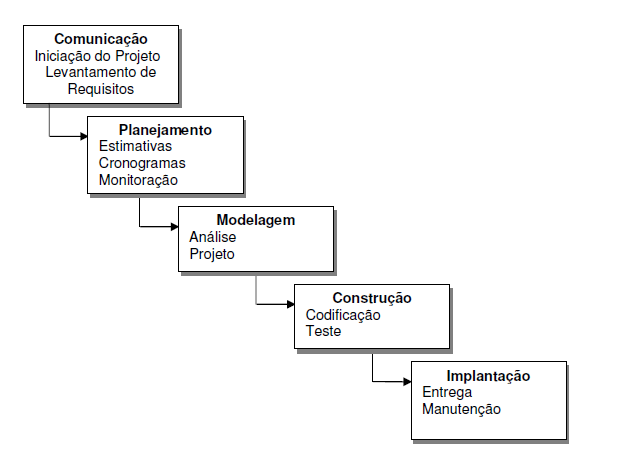
\includegraphics[width=7cm]{figuras/figura_ciclo_cascata}}
    }{
      \Fonte{\citeonline{pressman2006engenharia}}
    }	
\end{figure}


Dividimos o processo em nove atividades. A seguir, descreveremos brevemente cada uma delas:
\begin{alineascomnumero}
	\item \textbf{In\'icio do Projeto}: nessa atividade identificamos os objetivos do projeto e suas restri\c{c}\~oes.
	\item \textbf{Requisitos}: nessa atividade realizamos o levantamento e an\'alise dos requisitos, sua documenta\c{c}\~ao, verifica\c{c}\~ao e valida\c{c}\~ao, al\'em de um estudo para saber 
atrav\'es dos requisitos se o projeto \'e vi\'avel. 
	\item \textbf{Projeto}: nessa atividade desenvolvemos o projeto da arquitetura do sistema, o planejamento dos m\'odulos, o projeto da interface gr\'afica com o usu\'ario  e como ser\~ao 
persistidos as entidades do sistema.
	\item \textbf{Implementação}: nessa atividade escolhemos primeiramente um m\'odulo do sistema para implementar, em seguida planejamos como ocorrer\'a a implementa\c{c}\~ao desse 
m\'odulo, implementamos o m\'odulo, e por \'ultimo realizamos a integra\c{c}\~ao de m\'odulo ao resto do sistema. Esse ciclo \'e repetido at\'e que todos os m\'odulos estejam desenvolvidos.
	\item \textbf{Testes}: durante essa atividade realizaremos o planejamento dos testes para o sistema, em seguida executaremos os testes 
para cada m\'odulo do sistema e para o sistema como um todo, e por \'ultimo iremos gerar um relat\'orio com os resultados dos testes.
	\item \textbf{Implantação}: ap\'os o sistema desenvolvido e devidamente testado, ele segue para a implanta\c{c}\~ao, em que prepararemos 
o ambiente onde o sistema ser\'a executado e realizaremos a implanta\c{c}\~ao. Ap\'os a implanta\c{c}\~ao, realizaremos testes de 
aceita\c{c}\~ao e a cria\c{c}\~ao de um manual para o sistema.
	\item \textbf{Gerenciamento do Projeto}: essa atividade ocorre durante todo o desenvolvimento do sistema e tem por objetivo permitir que o projeto consiga ser conclu\'ido dentro do prazo e da 
qualidade desejada.
	\item \textbf{Avalia\c{c}\~ao do Processo}: essa atividade \'e executada durante todo o desenvolvimento do projeto e permite que o processo utilizado seja constantemente avaliado e adaptado 
conforme segue o desenvolvimento do projeto.
	\item \textbf{Encerramento do Projeto}: nessa \'ultima atividade ser\'a realizado apenas uma reuni\~ao em que ser\'a oficializado o final do projeto.
\end{alineascomnumero}

O processo desenvolvido est\'a dispon\'ivel em \url{www.askmath.quixada.ufc.br/static/process/}. 

\section{Levantamento e Análise de Requisitos}


O Levantamento e An\'alise de Requisitos é a fase do desenvolvimento de um \textit{software} em que o analista verifica junto ao usuário 
quais as necessidades, condições e princípios que o \textit{software} deverá atender \cite{matuda2013mapas}. Essa fase possibilitou 
conhecer e estudar as necessidades do cliente, assim como as restrições que o software estará sujeito.

Para realizar a coleta dos requisitos, optamos por utilizar entrevistas com o cliente, que no caso foi um dos professores de matemática da \gls{ufc}. Nessas entrevistas, que se caracterizaram como semi-estruturadas \footnote{Pois foram guiadas por um 
roteiro previamente elaborado e composto por questões abertas \cite{belei2008uso}}, foi possível obter os requisitos do sistema, assim como 
o público-alvo a quem o sistema atenderá. Essa técnica foi utilizada porque permitia uma organização flexível e ampliação dos 
questionamentos à medida que as informações foram sendo fornecidas pelo cliente \cite{fujisawa2000utilizaccao}.

O ambiente atender\'a quatro tipos de usu\'arios que formaram seu p\'ublico-alvo, ser\~ao administradores, professores, assistentes, e estudantes. Os administradores ser\~ao respons\'aveis por 
cadastrar novos professores, assim como realizar a manuten\c{c}\~ao do sistema. Os professores ser\~ao responsáveis por definir 
as disciplinas e li\c{c}\~oes que far\~ao parte do sistema. 
Ap\'os as disciplinas e li\c{c}\~oes serem definidas pelos professores, os assistentes ser\~ao respons\'aveis por manter\footnote{Adicionar, editar e excluir os problemas.} os problemas de cada 
li\c{c}\~ao. Os estudantes resolver\~ao os problemas desenvolvidos pelos assistentes e poder\~ao postar d\'uvidas sobre qualquer conte\'udo 
no f\'orum de discuss\~oes. Quando o ambiente for aplicado em sala de aula, os professores ser\~ao ainda respons\'aveis por gerenciar suas 
turmas e acompanhar o andamento do progresso de cada um de seus estudantes. J\'a os assistentes, ser\~ao responsáveis por tirar d\'uvidas 
dos estudantes no f\'orum de discuss\~oes.

Para uma melhor compreensão do público-alvo, foram criadas Personas \cite{pruitt2003personas}, personagens fictícios usados para 
caracterizar os papéis dos diferentes usuários do sistema \cite{guerra2010colaboraccao}. Cada Persona criada possui um nome, hábitos, 
histórias pessoais, motivações, objetivos, entre outras (ver \autoref{ap:personas}). A escolha dessa técnica deu-se pelo fato de que ela 
permite ao desenvolvedor saber mais precisamente para 
quem ele deveria construir o sistema, além de permitir uma distinção maior do público-alvo e, dessa forma, aprofundar-se nos interesses individuais de cada um.

Apresentaremos a seguir, os principais requisitos levantados durante essa etapa:

\begin{alineascomponto}
	\item Hierarquia dos Conteúdos: no sistema, dever\~ao existir disciplinas. Cada disciplina dever\'a possuir li\c{c}\~oes e cada li\c{c}\~ao ser\'a formada por problemas. Os professores poder\~ao 
cadastrar v\'arias disciplinas e li\c{c}\~oes, j\'a os assistentes ficar\~ao responsáveis por adicionar os problemas nas li\c{c}\~oes. Quando o estudante entrar no sistema, ele poder\'a ver somente 
as li\c{c}\~oes de uma disciplina por vez, podendo alternar entre disciplinas. Para um estudante come\c{c}ar a responder os problemas, ele dever\'a escolher inicialmente a disciplina e em seguida a 
li\c{c}\~ao. 

	\item Estrutura do Problema: cada problema possuir\'a uma descri\c{c}\~ao e v\'arios itens. Os problemas ser\~ao somente de m\'ultipla escolha e poder\~ao possuir no m\'inimo dois e no m\'aximo 
cinco itens. A quantidade de itens em cada problema ficar\'a a crit\'erio do assistente que adicionar\'a o problema ao sistema.

	\item Saltar Problemas: o sistema deverá permitir ao aluno saltar problemas e rever os saltos 
realizados com algumas restrições na quantidade de saltos..
	
	\item Pedir Ajuda: para todo problema, o estudante poderá consultar conte\'udo de ajuda. No momento em que o assistente estiver adicionando o problema, ele poderá ou não adicionar um texto de 
ajuda para o estudante, isso fica a critério dele. Quando o estudante estiver resolvendo os problemas, ele terá um botão que, quando acionado, mostrar\'a o texto de ajuda. O sistema dever\'a salvar a 
quantidade 
de vezes que o estudante pedir ajuda e em quais problemas.
	\item F\'orum: o sistema deverá possuir um fórum onde os estudantes possam postar suas dúvidas para que professores, assistentes e outro participantes possam lhes ajudar com o problema. Esse fórum, deve possuir tópicos, comentários para os tópicos, e os comentários devem oferecer a opção de se comentar com imagens.     

\end{alineascomponto}

Após o levantamento dos requisitos, foi realizada a análise dos mesmos. Nessa análise, os requisitos foram agrupados em categorias. As categorias utilizadas são descritas por 
\citeonline{sommerville2003engenharia} como:
\begin{alineascomponto}
    \item Requisitos Funcionais -- especificam ações que um sistema deve ser
capaz de executar, sem levar em consideração restrições físicas. Os requisitos
funcionais especificam, portanto, o comportamento de entrada e saída de um
sistema.
    \item Requisitos Não Funcionais -- descrevem apenas atributos do sistema ou
atributos do ambiente do sistema, como segurança, desempenho, usabilidade e
confiabilidade.
    \item Requisitos de Domínio -- são os requisitos do domínio da aplicação do sistema e que refletem características desse domínio.
\end{alineascomponto}

Após esse agrupamento, os requisitos funcionais foram representados em Casos de Uso \cite{jacobson92engenharia}. Um caso de uso identifica os agentes envolvidos em uma interação e especifica o tipo  de interação utilizando anotações sugeridas pela 
\gls{uml} \citeonline{sommerville2003engenharia}. Em seguida, foi realizada a documentação dos requisitos (ver \autoref{ap:requisitos}).

No final dessa etapa, ocorreu a Validação dos Requisitos junto ao cliente.  A Validação dos Requisitos é definida como o processo que certifica que o modelo de requisitos gerado  esteja  consistente  
com  as  necessidades  e  intenções  de  clientes  e usuários \cite{rilston2003metodologia}. Esta etapa permitiu que os requisitos coletados e documentados estivesse de acordo com o que o 
cliente solicitou.

\section{Projeto do Sistema}

O Projeto de Software é à atividade de engenharia cujo foco é definir ``como'' os requisitos estabelecidos no projeto devem ser implementados no software \cite{pressman2006engenharia}. O objetivo da  
atividade de projetar é gerar um modelo ou representação que apresente solidez, comodidade e deleite \cite{pressman2006engenharia}. Nesta fase, definimos como será aplicado o conhecimento obtido na 
pesquisa bibliográfica para se desenvolver o sistema. Para isto, definimos a arquitetura de software e as ferramentas que serão utilizadas durante o desenvolvimento do sistema. Nas seções a seguir, 
descrevemos um pouco sob cada um.

\subsection{Arquitetura}
Por arquitetura de software, entende-se a estrutura ou a organização de componentes de módulos, a maneira através da qual esses componentes interagem e a estrutura de dados que será usada pelos componentes \cite{pressman2006engenharia}.

A arquitetura utilizada baseia-se na arquitetura Cliente-Servidor\cite{david2013everything}, em que o processamento é dividido em processos distintos. Um processo é responsável pela manutenção da 
informação (servidor) e os outros são responsáveis pela captação de dados (clientes). Nessa arquitetura, os clientes enviam pedidos para o servidor, e este por sua vez processa estes dados e envia as 
respostas dos pedidos aos clientes.

Este modelo de arquitetura facilitará na manutenção do sistema, tendo em vista que toda atualização só necessitará ser realizada no servidor e automaticamente a mesma se propagará para todos os 
clientes. Com todos os recursos centralizados no servidor, podemos também ter um maior ganho com segurança, já que podemos centralizar os nossos esforços para manter a segurança das informações em 
apenas um único ponto, além de possibilitar que apenas cliente credenciados possam acessar e/ou alterar essas informações. Uma das outras grandes vantagens que temos  ao utilizar esse modelo, é que, 
\`a medida que a quantidade de clientes aumente, será possível suprir esses clientes sem necessitar realizar nenhuma modificação essencial.

Para uma visualização mais detalhada da arquitetura de \textit{software} definida, ver o  \autoref{ap:arquitetura}.

\subsection{Ferramentas}

A análise do sistema foi feita com o auxílio da ferramenta de criação de diagramas Astah \cite{astah2016}. A implementação com a linguagem 
Python \cite{vanrossum2010python}, o sistema de gerenciamento de banco de dados PostgresSQl \cite{momjian2001postgresql} e a camada de 
aplicação utilizar\'a o framework Django \cite{django2016}. O módulo Rosseta \cite{rosetta2016} ser\'a empregado 
para permitir a internacionalização do sistema.
 
A seguir, apresentaremos a lista das ferramentas e das tecnologias utilizadas para o desenvolvimento do projeto:

\begin{alineas}
	\item \textbf{Astah}: para a modelagem baseada em \acrshort{uml} do sistema.
	\item \textbf{Python}: linguagem de programação para implementação do sistema.
    \item \textbf{Django}: framework web responsável pela camada de aplicação.
    \item \textbf{Rosetta}: aplicação desenvolvida em Django que facilitará a tradução do projeto para diversas línguas.  
    \item \textbf{PostgreSQL}: como banco de dados para armazenamento e consulta de informações.
    \item \textbf{Metro UI CSS}: framework que faz uso de HTML, Cascading Stype Sheet (CSS) e Javascript para criação do front-end do sistema.
    \item \textbf{MathJax}: \'e uma engine\footnote{Uma biblioteca ou pacote de funcionalidades que são utilizadas para facilitar o desenvolvimento de alguma tecnologia.} de código aberto 
desenvolvido em 
javascript na forma de um plugin para incluir equações matemáticas em todos os navegadores, esse plugin aceita expressões em  MathML e Latex.

\end{alineas}

Algumas dessas ferramentas foram selecionadas por se tratarem de ferramentas \textit{Open Source}, ou seja, que seu código-fonte pode ser 
alterado para diferentes fins, possibilitando assim que qualquer um consulte, examine ou as modifique, e outras por serem ferramentas que 
possibilitam um rápido desenvolvimento.

No final dessa etapa, foi gerado o Plano de Projeto, documento que guiou o desenvolvedor durante todo o processo de desenvolvimento.

\section{Implementação do Sistema}

A implementação envolve as atividades de codificação, compilação e integração. A codificação visa traduzir o design num programa, utilizando linguagens e  ferramentas adequadas. A codificação 
deve refletir a estrutura e o comportamento descrito no projeto. Os componentes arquiteturais devem ser codificados de forma independente e depois integrados \cite{aguiar2012requisitos}.

O ambiente de desenvolvimento que est\'a sendo utilizado para desenvolver o sistema consiste em:
\begin{alineas}
	\item \textbf{Sistema Operacional}: Ubuntu 14.04 LTS;
	\item \textbf{Interpretador}: Python 2.7.6;
	\item \textbf{Banco de Dados}: PostgreSQL 9.3.13;
	\item \textbf{\textit{Framework} de \textit{back-end}}: Django 1.7.11;
	\item \textbf{\textit{Framework} de \textit{front-end}}: Metro UI CSS 3.0.15;
\end{alineas}

Para permitir uma maior independ\^encia desse ambiente com a maquina em que estamos desenvolvendo o sistema, decidimos criar um ambiente de desenvolvimento com o auxilio da 
ferramenta Virtualenv 15.0.2. O Virtualenv permite isolar o ambiente de desenvolvimento de um determinado projeto para garantir que um pacote instalado não interfira nos demais projetos que 
rodam na maquina, al\'em de possibilitar saber facilmente a vers\~ao de todos os pacotes e componentes que est\~ao sendo utilizados para desenvolver o sistema. Essa informa\c{c}\~ao \'e 
importante quando formos replicar o ambiente de desenvolvimento no servidor de produ\c{c}\~ao\footnote{O ambiente de produção é onde os usuários finais acessarão o software}. 

Todos os c\'odigos-fonte gerados nessa etapa, passaram por um processo de versionamento\footnote{O versionamento de uma aplicação tem como 
foco principal documentar as inclusões, alterações ou até mesmo exclusões de funcionalidades.} atrav\'es da ferramenta Git 1.9.1, 
essa ferramenta permite:

\begin{alineascomponto}
	\item \textbf{Controle do histórico}: facilidade em desfazer e analisar o histórico do desenvolvimento, como também facilidade no resgate de versões mais antigas e estáveis.
	\item \textbf{Marca\c{c}\~ao e Resgate de Vers\~oes Est\'aveis}: permite marca onde um documento estava com uma vers\~ao est\'avel, para ser facilmente resgatado no futuro.
	\item \textbf{Ramifica\c{c}\~ao do Projeto}: permite dividir o projeto em v\'arias linhas de desenvolvimento sem que uma interfira na outra. 
\end{alineascomponto}

No final dessa etapa, tivemos os código-fonte de todos os módulos do sistema, assim como o próprio sistema em funcionamento. 

\section{Verificação e Validação}
Essa etapa destinou-se a mostrar que o sistema está de acordo com a especificação e que ele atende às expectativas de clientes e usuários, al\'em de assegurar que o  programa está fazendo aquilo que foi definido na sua especificação e que não possui  erros  de execução \cite{aguiar2012requisitos}. 

Durante essa fase, realizamos Testes de Unidade e Integra\c{c}\~ao em cada modulo do sistema, assim como Testes de Sistema no sistema j\'a integrado.

\citeonline{aniche2014teste} define essas categorias de Testes de Software como:

\begin{alineascomponto}
	\item \textbf{Teste de Unidade} -- é aquele que testa uma única unidade do sistema. Ele a testa de maneira isolada, geralmente simulando as 
prováveis dependências que aquela unidade tem. Em sistemas orientados a objetos, é comum que a unidade seja uma classe. Ou seja, quando 
queremos escrever testes de unidade para a classe Pedido, essa bateria de testes testará o funcionamento da classe Pedido, 
isolada, sem interações com outras classes.
	\item \textbf{Teste de Integração} -- é aquele que testa a integração entre duas partes do seu sistema. Os testes que você escreve para a sua 
classe PedidoDao, por exemplo, em que seu teste vai até o banco de dados, é um teste de integração. Afinal, você está testando a integração 
do seu sistema com o sistema externo, que é o banco de dados. Testes que garantem que suas classes comunicam-se bem 
com serviços web, escrevem arquivos texto, ou mesmo mandam mensagens via \textit{socket} são considerados testes de integração.
	\item \textbf{Teste de Sistema} -- \'e aquele que garante que o sistema funciona como um todo. Este 
nível de teste está interessado se o sistema funciona como um todo, com todas as 
unidades trabalhando juntas. Ele é comumente chamado de teste de caixa preta, já 
que durante o teste n\~ao se importa com a forma que os dados s\~ao processados, mas sim se as sa\'idas est\~ao de acordo com o que era esperado para entradas. 
\end{alineascomponto}

\section{Definição dos Conteúdo para o Sistema}

Após o sistema estar verificado e validado, ele teve que possuir conteúdos para ser utilizado por usu\'ario durante os testes com usu\'arios. Decidimos optar por deixar os monitores\footnote{É o aluno de graduação concursado para exercer, juntamente com o professor, atividades técnico-didáticas condizentes com o seu grau de conhecimento junto à determinada disciplina, já por ele cursada.} das turmas de matemática desenvolverem os conteúdos que foram utilizados no sistema durante a fase de avaliação. 

Os monitores passaram por um treinamento, no qual aprenderam a utilizar o sistema para adicionarem os conteúdos.
	\chapter{RESULTADOS}
\label{chap:resultados}

Nesta seção apresentaremos o resultado deste trabalho.

Definimos o processo que foi utilizado durante o desenvolvimento do sistema, coletamos, analisamos e validamos os requisitos do sistema e realizamos o projeto do sistema. 

Na implementação, desenvolvemos os módulos: 

\begin{alineascomponto}
    \item Gerenciador de Usuários: módulo responsável por gerenciar os usuários do sistema como professores, assistentes e alunos.
    \item Gerenciador de Turmas: módulo responsável por gerenciar as turmas de alunos do sistema.
    \item Gerenciador de Disciplinas: módulo responsável por gerenciar as disciplinas que serão cadastradas no sistema.
    \item Gerenciador de Lições: módulo responsável por gerenciar as lições que os professores irão cadastrar no sistema.
    \item Gerenciador de Questões: módulo responsável por gerenciar os problemas que os assistentes e professores poderão cadastrar para cada lição.
    \item Gerenciador de Pontuação: módulo responsável por gerenciar a pontuação ganha pelos alunos, assim como seu nível de experiência ao longo da utilização do sistema. 
    \item Fórum: módulo responsável por permitir que alunos postem dúvidas dos mais variados  assuntos relacionadas ao sistema, seja dúvidas em relação ao conteúdo apresentado em sala de aula, assim como informações sobre o sistema e sugestões.
    \item Gerenciador de Progresso: módulo responsável por acompanhar o andamento de cada estudante durante seu aprendizado e identificar os obstáculo epistemológicos enfrentados, indicando ao aluno 
a exist\^encia desses obst\'aculos e o(s) conte\'udo(s) que ele possui defici\^encia (causador(es) do obstáculo) para ele assim poder pausar o conte\'udo que est\'a estudando e voltar a 
estudar o(s) conte\'udo(s) que o sistema indicar.
	\item Gerador de Estatísticas: módulo responsável por gerar as estatísticas que o professor utilizará para acompanhar o andamento de suas turmas e alunos, assim como para o uso pelo estudante, 
que utilizará para acompanhar seu próprio progresso durante sua aprendizagem no sistema. 
\end{alineascomponto}

A seguir, apresentaremos algumas telas do sistema:

\begin{figure}[h!]
  \centering
  \begin{minipage}[b]{0.49\textwidth}
	\caption{Tela Inicial}
    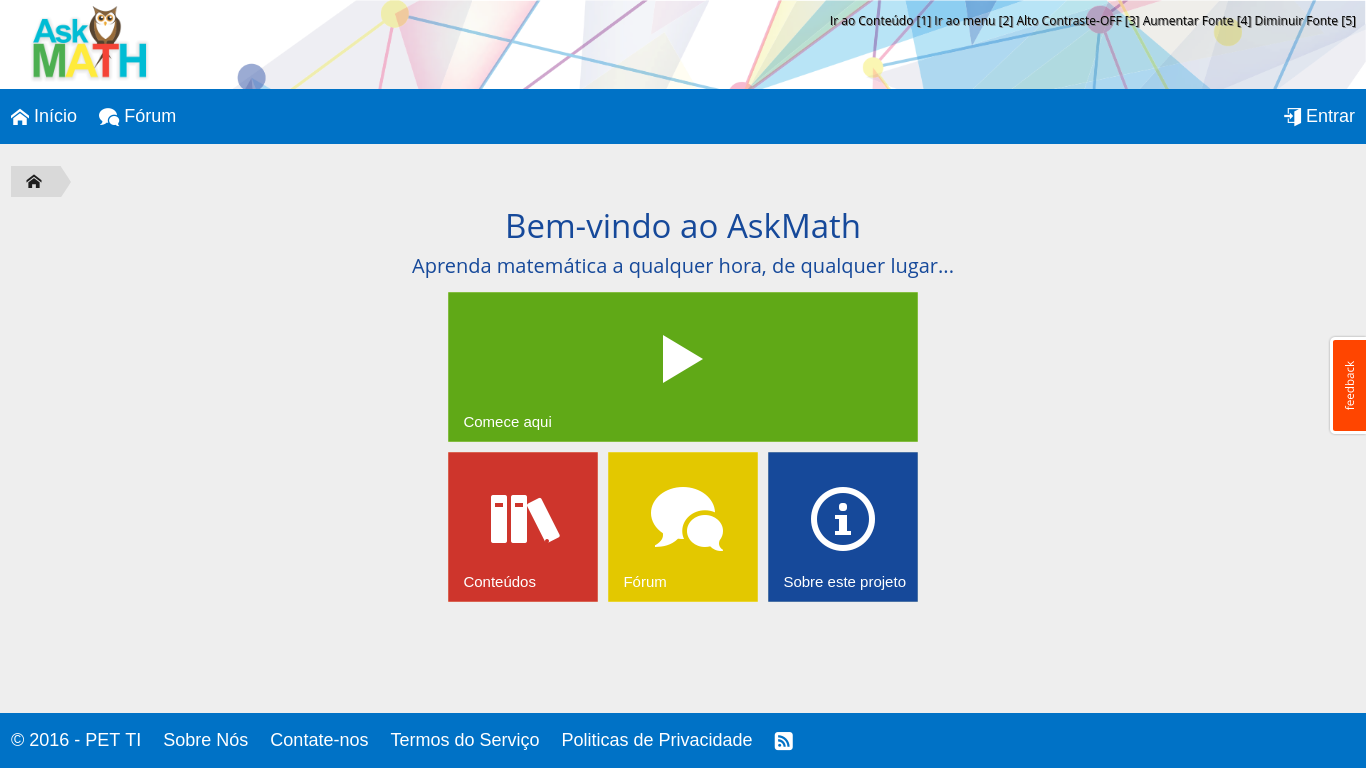
\includegraphics[width=\textwidth]{figuras/askmath/1}
  \end{minipage}
  \hfill
  \begin{minipage}[b]{0.49\textwidth}
	\caption{Tela Inicial do Estudante}
    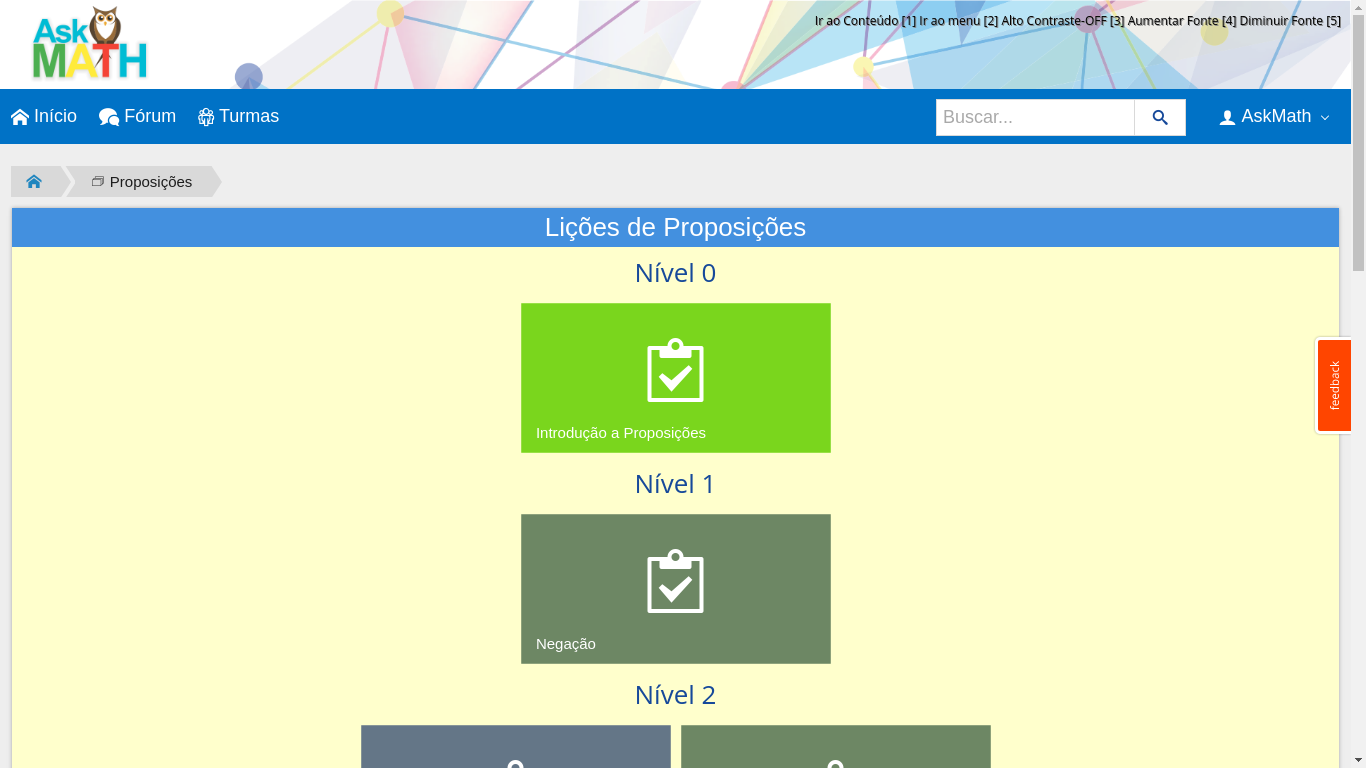
\includegraphics[width=\textwidth]{figuras/askmath/2}
  \end{minipage}
 
  \begin{minipage}[b]{0.49\textwidth}
    \caption{Tela de Administra\c{c}\~ao}
    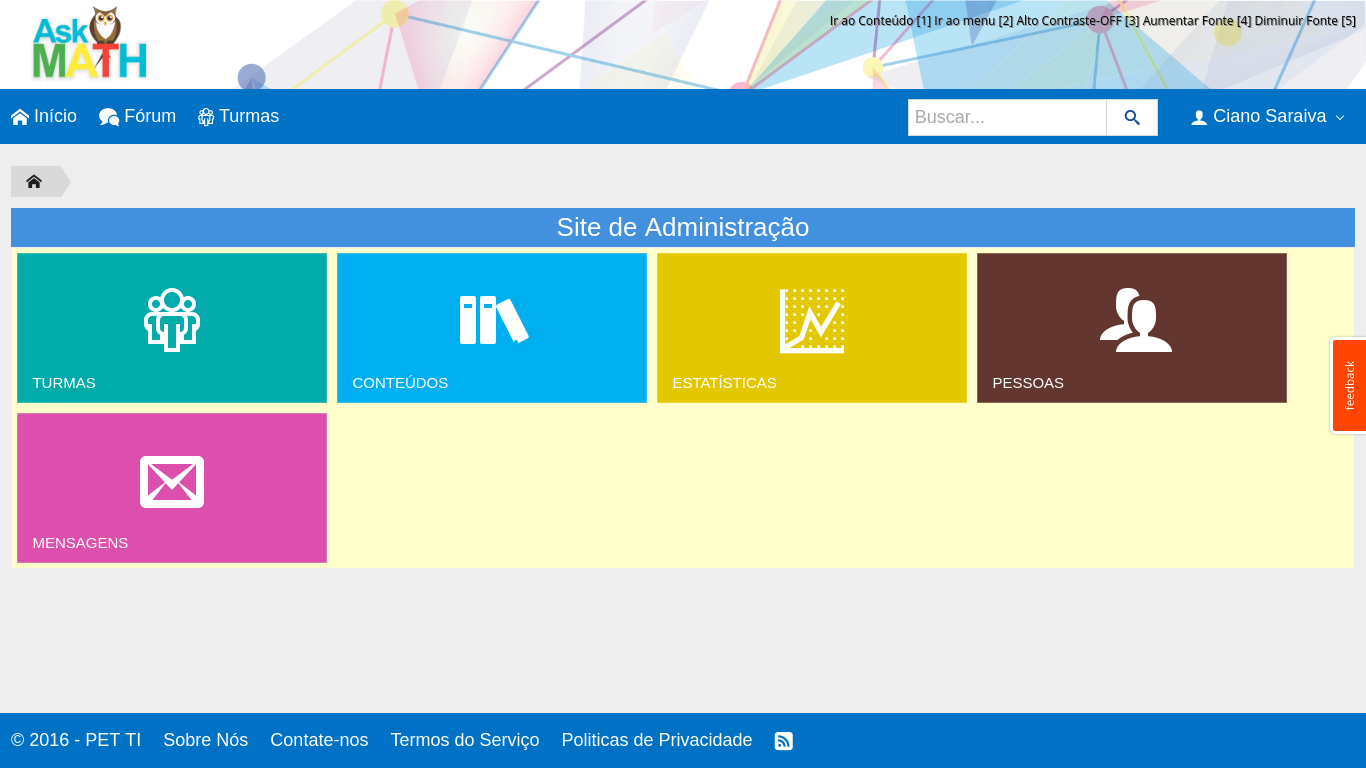
\includegraphics[width=\textwidth]{figuras/askmath/3}
  \end{minipage}
  \hfill
  \begin{minipage}[b]{0.49\textwidth}
	\caption{Tela de Problemas do Estudante}
    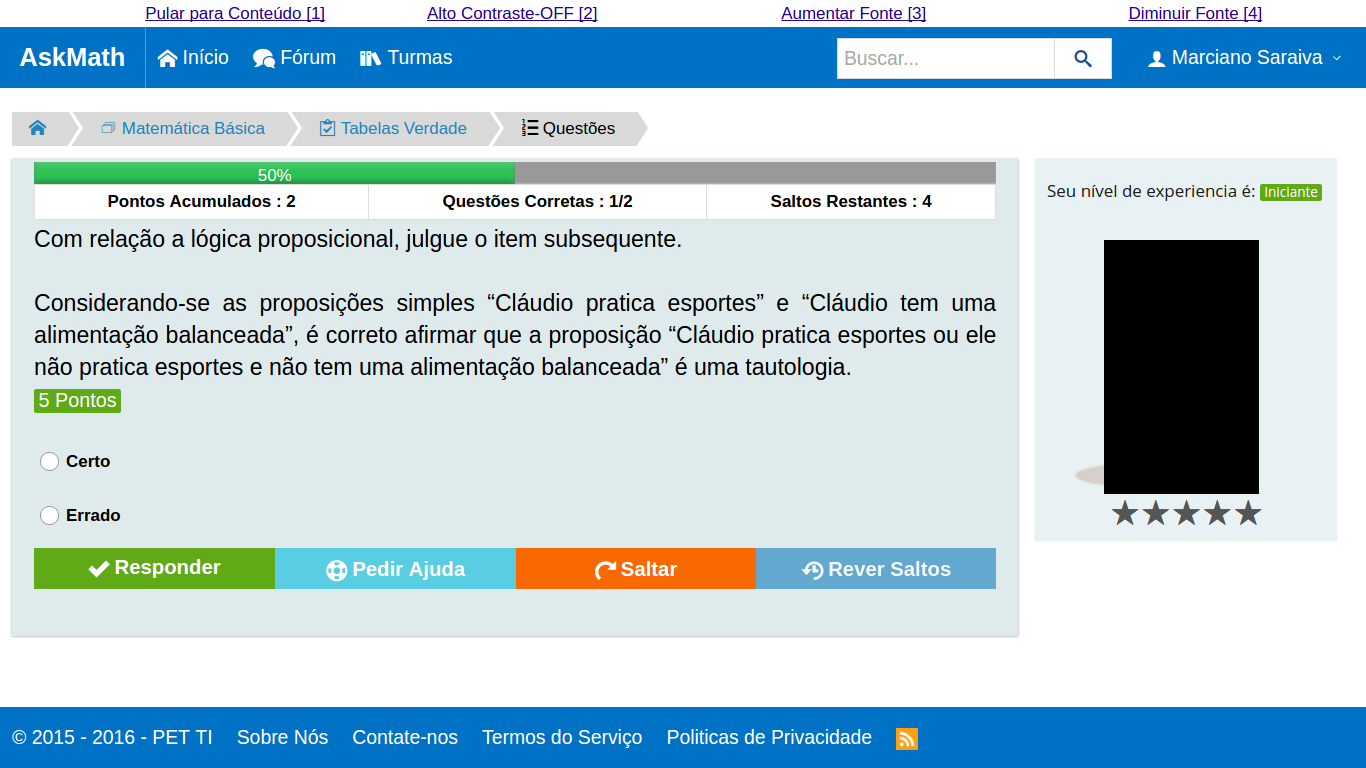
\includegraphics[width=\textwidth]{figuras/askmath/4}
  \end{minipage}
\end{figure}

[FALAR DA AVALIAÇÂO AQUI]
	\chapter{CONCLUSÕES E TRABALHOS FUTUROS}
\label{chap:conclusoes-e-trabalhos-futuros}

Esse capítulo apresenta as considerações finais a cerca desse trabalho. Além disso, é proposta a inclusão de novas funcionalidades que podem ser desenvolvidas em trabalhos futuros.

\section{Conclusões}

Após a implementação da solução proposta por este trabalho, constatou-se que tanto o objetivo geral quanto os específicos foram atendidos. O sistema foi desenvolvido conforme as melhores práticas e padrões em desenvolvimento de \textit{software} disponíveis no momento, tornando o sistema flexível, modularizado e reusável. Além disso, o sistema proporciona de fato um ambiente em que alunos podem práticar os conhecimentos adquiridos e até assimilar novos conhecimento. 

Finalmente, o sistema pode ainda ser utilizado como complemento ao ensino presencial, auxiliando professores e tutores no acompanhamento do aprendizado de seus alunos e apredizes.

Podem-se evidenciar limitações na solução desenvolvida na questão da comunicação entre aluno-aluno e aluno-profesor, já que isso só ocorre através do fórum de discurções, vale ressaltar que é improvável que, durante a aplicação do sistema, tais limitações sejam atingidas a ponto de comprometer a finalidade do sistema.

\section{Sugestões para Trabalhos Futuros}

No que tange trabalhos futuros que podem ser realizados baseando-se neste projeto, podem ser citados: desenvolver um módulo de bate-papo entre os alunos e professores, adição de conteúdos apresentados através de recursos visuais como vídeo, melhorias na \textit{interface} gráfica para aumentar a usabilidade do sistema. 

Por fim, pode-se avaliar o aprendizado que o sistema pode proporcionar à alunos durante seu uso como complemento ao ensino.




	
	%Elementos pós-textuais	
	\bibliography{elementos-pos-textuais/referencias}
	\imprimirglossario
	\imprimirapendices
		% Adicione aqui os apendices do seu trabalho
 		\apendice{\textbf{DOCUMENTO DE PERSONAS}}\label{ap:personas}
\addtocontents{toc}{\protect\setcounter{tocdepth}{0}}

\section{Charlie - Técnico em Informática}

\begin{figure}[h!]
  \centering
  \Caption{\label{fig:persona_1} Imagem de Charlie}	
  \UFCfig{}{
    \fbox{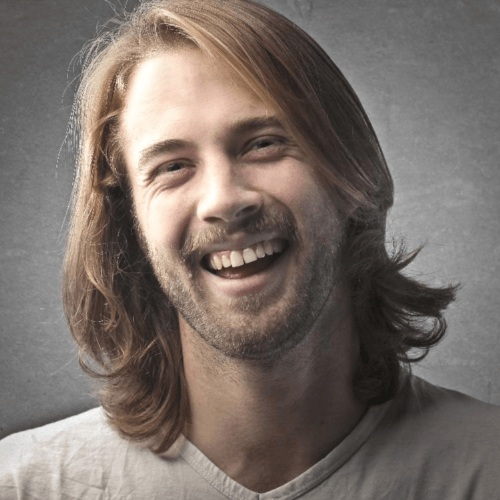
\includegraphics[width=6cm]{figuras/personas/figura_persona_1}}
  }{
    \Fonte{\url{www.geradordepersonas.com.br}}
  }	
\end{figure}

Empresa: Charlie trabalha na TechSolutions, uma empresa de tecnologia pequena, mas que está ganhando
clientes e ampliando seus negócios.

Idade: 24 anos.

Genêro: Masculino.

Educação: Ensino técnico.

Mídias: Lê a revista Exame e usa ativamente email para trocar informações com 
outros funcionários da empresa.

Objetivos: Como a empresa que Charlie trabalha está ampliando seus negócios, ela
necessita que alguns de seus funcionários possuam um melhor conhecimento na 
área, por isso, Charlie decidiu investir num ensino superior. O objetivo de Charlie é 
concluir seu curso de Engenharia de Software e voltar a trabalhar normalmente 
para sua empresa.

Desafios: Charlie está com muita dificuldade na primeira disciplina de Matemática de seu curso. Como ele já concluiu o ensino médio há bastante tempo, ele não se lembra de como resolver 
questões simples de matemática como funções de 1º grau, 2º grau, racionais, entre outras. Ele começou a estudar, mas 
não consegue encontrar uma forma intuitiva para verificar se está indo bem nos 
seus estudos, ficando preso aos exercícios que ele encontra nos livros.

Como podemos ajudá-lo: O AskMath possibilitará que Charlie estude 
todos os conteúdos que ele j\'a havia estudado no ensino médio e que já os tinha esquecido. São lições agrupadas por disciplina, cada lição possui um conjunto de problemas criados especialmente para 
pessoas com dificuldade em aprender. Nosso sistema possibilitará que Charlie veja instantaneamente se sua resposta é correta ou não, ele também poderá pedir ajuda 
e saltar quest\~oes caso o mesmo não se sinta a vontade para respondê-las naquele 
momento. Com isso, é possível que ele acompanhe através de estatísticas como 
está seu desempenho durante os estudos.

\section{Ruby - Bolsista de Graduação}

\begin{figure}[h!]
  \centering
  \Caption{\label{fig:persona_2} Imagem de Ruby}	
  \UFCfig{}{
   \fbox{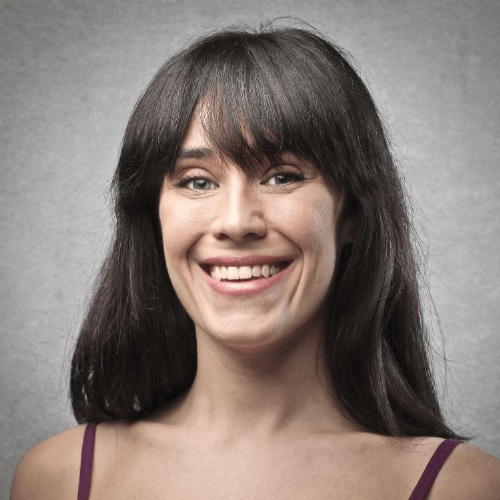
\includegraphics[width=6cm]{figuras/personas/figura_persona_2}}
  }{
    \Fonte{ \url{www.geradordepersonas.com.br} }
  }	
\end{figure}


Empresa: Ruby trabalha como bolsista de monitoria das disciplinas envolvendo 
Matemática na Universidade Federal do Ceará.

Idade: 21 anos.

Genêro: Feminino.

Educação: Ensino superior.

Mídias: Usa ativamente o facebook, twitter e wattsapp.

Objetivos: O principal objetivo de Ruby é terminar sua graduação e tentar uma 
bolsa de mestrado numa universidade renomada.

Desafios: Ruby como monitora das disciplinas de matemática, não consegue se
aproximar dos alunos para ajuda-los com suas dúvidas. Segundo ela, "eles tem medo de 
dizer para nós monitores que est\~ao com dificuldades", então Ruby está em busca de 
novas formas de ajudar os estudantes que estão com dificuldades.

Como podemos ajudá-la: Com o AskMath, Ruby poderá ajudar esses alunos adicionando problemas para eles exercitarem seus conhecimentos e tirar suas d\'uvidas no f\'orum de discuss\~ao que 
o sistema oferece.

\section{Samuel - Professor}

\begin{figure}[h!]
  \centering
  \Caption{\label{fig:persona_3} Imagem de Samuel}	
  \UFCfig{}{
   \fbox{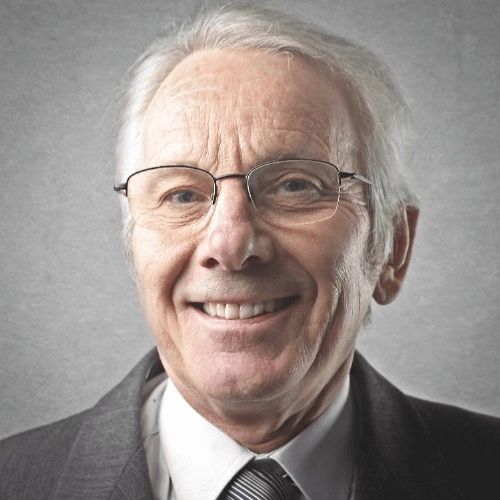
\includegraphics[width=6cm]{figuras/personas/figura_persona_3}}
  }{
    \Fonte{ \url{www.geradordepersonas.com.br} }
  }	
\end{figure}

Empresa: Samuel trabalho como professor da disciplina de C\'alculo I na
Universidade Federal do Ceará.

Idade: 59 anos.

Genêro: Masculino.

Educação: Doutorado.

Mídias: Lê o jornal The New York Times e usa email para tirar dúvidas dos alunos.

Objetivos: Samuel é um professor exemplar e se preocupa muito em ensinar seus 
alunos. Seu principal objetivo é ensinar da melhor forma possível seus alunos, 
de forma que todos possam seguir excelentes carreiras quando se formar e se 
tornem ótimos profissionais.

Desafios: Samuel gosta de acompanhar o andamento dos estudos de seus alunos. Quando Samuel os questionam sobre as dificuldade que eles est\~ao enfrentando nos seus estudos, os mesmos dizem que ``está 
tudo bem'', o que não reflete em suas notas. Sabendo disso, Samuel fica triste, já que não consegue saber como anda os estudos de seus alunos e gostaria de ajudá-los ainda mais.

Como podemos ajudá-lo: Com o AskMath, Samuel poder\'a acompanhar o andamento de sua turma e saber em quais conteúdos os alunos est\~ao com mais dificuldade, para dar uma aten\c{c}\~ao especial a 
esses conte\'udos. Samuel poderá ainda adicionar os conteúdos que ele achar mais interessantes, para que seus alunos possam praticar os conhecimentos adquiridos em sala de aula no conforto de suas 
casas. Samuel tamb\'em ver\'a as dúvidas que os alunos postam no fórum de discuss\~oes e quais desses alunos est\~ao enfrentando obstáculos durante sua aprendizagem.

\section{Stefane - Estudante do Ensino Médio}

\begin{figure}[h!]
  \centering
  \Caption{\label{fig:persona_4} Imagem Stefane}	
  \UFCfig{}{
   \fbox{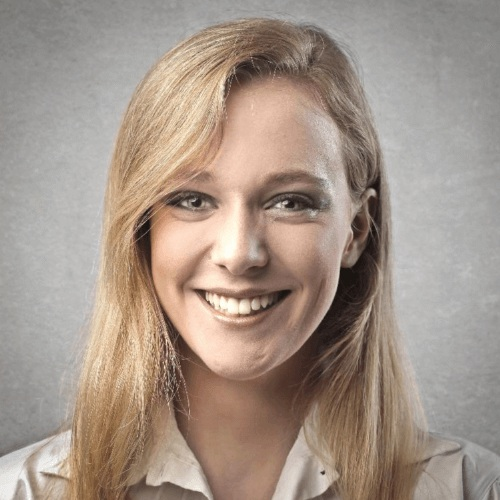
\includegraphics[width=6cm]{figuras/personas/figura_persona_4}}
  }{
    \Fonte{ \url{www.geradordepersonas.com.br} }
  }	
\end{figure}



Empresa: Ela trabalha no salão de beleza de sua mãe.

Idade: 18 anos.

Genêro: Feminino.

Educação: Ensino médio.

Mídias: Usa ativamente o facebook e WatssApp.

Objetivos: Stefane busca concluir o ensino médio e tirar uma boa nota no ENEM 
para tentar conseguir uma vaga para cursar Sistemas de Informação na Universidade Federal do Cear\'a, que é 
o curso de seus sonhos.

Desafios: Stefane, como estudante, não gosta de estudar matemática por livros e acha incomodo ter que levar seus livros enormes de matemática em sua bolsa para o salão de beleza de sua mãe para 
estudar, mas tamb\'em quer ficar estudando enquanto não aparece clientes no salão. Um outro problema de Stefane, é que às vezes, ela fica com dúvidas na resolução de algum problema e precisa ligar 
para seus amigos em busca de explicações que nem sempre encontra.

Como podemos ajudá-la: Com o AskMath, Stefane não precisará mais levar seus livros de Matemática em sua bolsa, para aprender matemática ela precisar\'a apenas de uma celular e isso possibilita que 
ela possa continuar estudando no salão enquanto este estiver vazio. Para solucionar as dúvidas de Stefane, 
temos pessoas esperando para ajudá-la no f\'orum de discuss\~ao, em que ela pode compartilhar suas d\'uvidas para que outros estudantes e professores possam ajuda-la e ao mesmo tempo ajudar outros 
que estejam com a mesma d\'uvida de Stefane. 

\addtocontents{toc}{\protect\setcounter{tocdepth}{1}}
		\apendice{\textbf{DOCUMENTO DE REQUISITOS}}\label{ap:requisitos}
\addtocontents{toc}{\protect\setcounter{tocdepth}{0}}

\section{Introdução}
Este documento especifica os requisitos do sistema AskMath, fornecendo aos desenvolvedores as informações necessárias para o projeto e implementação, assim como para a realização dos testes. 

\subsection{Visão geral do documento}
Este documento apresenta os requisitos funcionais, n\~ao funcionais e de domínio.Para cada da requisito funcional, definimos seu caso de uso e sua descrição detalhada. Além disso, definimos sua 
prioridade, explicado no tópico abaixo, e suas pré e pós condições, entradas e saídas caso existam, e por fim os diagramas de casos de uso do sistema e seus detalhamentos.

\subsection{Prioridades dos requisitos}
Cada requisito terá uma determinada prioridade, essa prioridade ira ajudar a equipe de desenvolvimento na escolha de quais requisitos mais se preocupar quando tiver desenvolvendo o sistema, criamos para isso, três níveis prioridades:

\begin{alineascomponto}
	\item \textbf{Essencial}: é o requisito ao qual o sistema não entra em funcionamento sem ele. Esses requisitos tem que ser implementados o mais rápido possível. 
    \item \textbf{Importante}: requisito sem o qual o sistema entra em funcionamento, mas de forma não satisfatória. Esse requisitos deverão sem implementados, mas caso não sejam, o sistema ainda 
poderá funcionar consideravelmente.
	\item \textbf{Desejável}: requisito que não compromete o sistema, esse tipo de requisito é comumente deixado para versões posteriores do sistema.
\end{alineascomponto}

\section{Requisitos Funcionais}

\noindent
\fbox{
\parbox{\textwidth}{
  \begin{center}
    [RF001] Tipos de Usuário e Autenticação
  \end{center}
  
  O Sistema deverá possuir quatro tipos usuários, são estudantes, assistentes, professores e administradores, e todos deverão ser autenticados. O sistema deverá possuir um procedimento de autorização de utilizadores, onde cada utilizador deverá se identificar através de um nome de usuário e uma senha. Apenas os utilizadores autorizados podem acessar o sistema.
  \linebreak
  Prioridade: Essencial
}}

\noindent
\fbox{
\parbox{\textwidth}{
  \begin{center}
  [RF002] Cadastro
  \end{center}
Para administradores, professores ou assistentes realizarem seu cadastro no sistema, será necessário que um administrador ou professor já com acesso ao sistema gere uma chave de acesso que poderá ser usada para permitir o cadastro. Caso o usuário não tenha essa chave de acesso, sua única opção para cadastro é a opção de estudante. 
\linebreak
Prioridade: Essencial
}}

\noindent
\fbox{
\parbox{\textwidth}{
  \begin{center}
  [RF003] Recuperar Senha
  \end{center}
O Sistema deverá propiciar aos usuário uma opção para recuperar sua senha caso necessite.
\linebreak
Prioridade: Essencial
}}

\noindent
\fbox{
\parbox{\textwidth}{
  \begin{center}
	[RF004] Hierarquia dos Conteúdos
  \end{center}
No sistema, dever\~ao existir disciplinas, cada disciplina dever\'a possuir li\c{c}\~oes e cada li\c{c}\~ao ser\'a formada por problemas. Os professores poder\~ao 
cadastrar v\'arias disciplinas e li\c{c}\~oes, j\'a os assistentes ficar\~ao responsáveis por adicionar os problemas nas li\c{c}\~oes. Quando o estudante entrar no sistema, ele poder\'a ver somente 
as li\c{c}\~oes de uma disciplina por vez, podendo alternar entre disciplinas. Para um estudante come\c{c}ar a responder os problemas, ele dever\'a escolher inicialmente a disciplina e em seguida a 
li\c{c}\~ao. 
\linebreak
Prioridade: Essencial
}}

\noindent
\fbox{
\parbox{\textwidth}{
  \begin{center}
	[RF005] Estrutura do Problema
  \end{center}
Cada problema possuir\'a uma descri\c{c}\~ao e v\'arios itens. Os problemas ser\~ao somente de m\'ultipla escolha e poder\~ao possuir no m\'inimo dois e no m\'aximo 
cinco itens, essa quantidade ficar\'a a crit\'erio do assistente que realizar\'a a adi\c{c}\~ao do problema no sistema.
\linebreak
Prioridade: Essencial
}}

\noindent
\fbox{
\parbox{\textwidth}{
  \begin{center}
	[RF006] Manter Disciplinas
  \end{center}

Professores poderão adicionar, editar e excluir disciplinas e lições.
\linebreak
Prioridade: Essencial
}}

\noindent
\fbox{
\parbox{\textwidth}{
  \begin{center}
	[RF007] Manter Problemas
  \end{center}
Assistentes poderão adicionar, editar e excluir problemas das lições.
\linebreak
Prioridade: Essencial
}}

\noindent
\fbox{
\parbox{\textwidth}{
  \begin{center}
	[RF008] Alternar entre Disciplinas
  \end{center}
Quando o aluno entrar no sistema pela primeira vez, ele verá uma lista com as 
disciplinas disponíveis, ele então deverá escolher uma opção. Em seguida, irão 
aparecer apenas lições referentes aquela disciplina, mas, caso ele queira, ele 
poderá trocar facilmente de disciplina.
\linebreak
Prioridade: Essencial
}}

\noindent
\fbox{
\parbox{\textwidth}{
  \begin{center}
	[RF009] Ver Detalhes da Lição
  \end{center}
Antes de começar a resolver os problemas de uma lição, o estudante deverá ver informações sobre a mesma.
\linebreak
Prioridade: Essencial
}}

\noindent
\fbox{
\parbox{\textwidth}{
  \begin{center}
	[RF010] Sair da Lição
  \end{center}
O Aluno poderá sair da lição antes mesmo de tê-la concluído, voltando depois à 
posição onde parou. Ao sair, o aluno deverá ver estatísticas referentes a 
evolução dele na lição.
\linebreak
Prioridade: Essencial
}}

\noindent
\fbox{
\parbox{\textwidth}{
  \begin{center}
	[RF011] Saltar Problemas
  \end{center}
O sistema deverá permitir ao aluno saltar problemas e rever os saltos 
realizados com algumas restrições na quantidade de saltos.
\linebreak
Prioridade: Essencial
}}

\noindent
\fbox{
\parbox{\textwidth}{
  \begin{center}
	[RF012] Pedir ajuda
  \end{center}
Para todo problema, o estudante poderá possuir uma ajuda. No momento em que o assistente estiver adicionando o problema, ele poderá ou não adicionar um texto de ajuda para o 
estudante, isso fica a critério dele. Quando o estudante estiver resolvendo os problemas, ele terá um botão que quando acionado, mostrar\'a o texto de ajuda. O sistema dever\'a salvar a quantidade 
de vezes que o estudante pedir ajuda e em quais problemas.  
\linebreak
Prioridade: Essencial
}}

\noindent
\fbox{
\parbox{\textwidth}{
  \begin{center}
	[RF013]  Alterar Visibilidade do Problema
  \end{center}
Um problema pode ser visível aos estudantes ou não. Quando o assistente estiver 
adicionando um problema, terá um campo marcado por padrão como verdadeiro que 
indicará se o problema estará visível ou não para os alunos. Caso o mesmo não 
queira que o problema adicionado fique imediatamente visível aos alunos, ele 
desmarcar\'a esse campo e futuramente ele poderá editar o problema e marcá-lo 
quando quiser que os alunos possam acessá-la.
\linebreak
Prioridade: Essencial
}}

\noindent
\fbox{
\parbox{\textwidth}{
  \begin{center}
	[RF014] Deficiências
  \end{center}
É possível, a partir de um item respondido incorretamente em um problema, identificar a deficiência do estudante, por isso é fundamental que no momento que o 
assistente estiver adicionando os itens do problema, ele possa escolher para cada item incorreto, uma ou várias li\c{c}\~oes, essas lições ficarão sendo as supostas deficiências do aluno caso ele 
responda incorretamente aquele problema marcando aquele determinado item.
\linebreak
Prioridade: Essencial
}}

\noindent
\fbox{
\parbox{\textwidth}{
  \begin{center}
	[RF015] Recompensas e Punições
  \end{center}
A cada 3 problemas que o aluno responder corretamente, ele será parabenizado e 
ganhará um prêmio e a cada 3 errados ele será penalizado. Quando o aluno 
resolver seguidamente três problemas corretamente, os seus pontos acumulados 
irão dobrar e a cada vez que ele errar três questões seguidamente, seus pontos 
acumulados serão subtraídos em 25%.
\linebreak
Prioridade: Essencial
}}

\noindent
\fbox{
\parbox{\textwidth}{
  \begin{center}
	[RF016] Fórum
  \end{center}
O sistema deverá possuir um fórum onde os estudantes possam postar suas dúvidas para que professores, assistentes e outro participantes possam lhes ajudar com o problema. Esse fórum, deve possuir tópicos, comentários para os tópicos, e os comentários devem oferecer a opção de se comentar com imagens.
\linebreak
Prioridade: Essencial
}}

\noindent
\fbox{
\parbox{\textwidth}{
  \begin{center}
	[RF017] Ordenar Problemas
  \end{center}
O Sistema deve apresentar ao assistente uma forma simples para ele ordenar a 
sequência dos problemas de cada lição.
\linebreak
Prioridade: Essencial
}}

\noindent
\fbox{
\parbox{\textwidth}{
  \begin{center}
	[RF018] Suporte a Latex
  \end{center}
O Sistema deve permitir ao assistente adicionar código Latex na criação 
dos problemas e lições. Quando os assistentes adicionarem os problemas, o sistema 
devera reconhecer código Latex referente a fórmulas matemáticas. Toda vez que o assistente colocar um código Latex entre duas tags '\$', o sistema deverá reconhecer isso e mostrar para o usuário a imagem da fórmula referente àquele código.
\linebreak
Prioridade: Essencial
}}


\section{Requisitos N\~ao Funcionais}

\noindent
\fbox{
\parbox{\textwidth}{
  \begin{center}
	[RN001] Tecnologias
  \end{center}
O Sistema deve ser desenvolvido apenas com tecnologias open source.
\linebreak
Prioridade: Essencial
}}

\noindent
\fbox{
\parbox{\textwidth}{
  \begin{center}
	[RN002] Persistência dos Dados
  \end{center}
O sistema deverá utilizar como sistema de gerenciamento de banco de dados o 
PostgreSQL.
\linebreak
Prioridade: Importante
}}

\noindent
\fbox{
\parbox{\textwidth}{
  \begin{center}
	[RN003] Segurança
  \end{center}
O sistema não apresentará aos usuários quaisquer dados de cunho privativo.
\linebreak
Prioridade: Essencial
}}

\noindent
\fbox{
\parbox{\textwidth}{
  \begin{center}
	[RN004] Estrutura
  \end{center}
O sistema deverá ser desenvolvido de forma modular para permitir a reusabilidade de seus módulos por outras aplicações no futuro. 
\linebreak
Prioridade: Essencial
}}

\noindent
\fbox{
\parbox{\textwidth}{
  \begin{center}
	[RN005] Padrões
  \end{center}
O Sistema deverá ser desenvolvido utilizando os princípios de Orientação a 
Objetos.
\linebreak
Prioridade: Essencial
}}

\noindent
\fbox{
\parbox{\textwidth}{
  \begin{center}
	[RN006] Ambiente de Execução
  \end{center}
O sistema deverá ser acessado completamente via browser HTTP/HTML. 
\linebreak
Prioridade: Essencial
}}

\noindent
\fbox{
\parbox{\textwidth}{
  \begin{center}
	[RN007] Acessibilidade
  \end{center}
O Sistema devera possuir Responsive Web Design, assim como as v\'arias 
diretivas de acessibilidade para web.
\linebreak
Prioridade: Importante
}}

\noindent
\fbox{
\parbox{\textwidth}{
  \begin{center}
	[RN008] Internacionalização
  \end{center}
O Sistema será disponibilizado em inglês, mas de forma a permitir que versões em 
línguas latinas possam ser produzidas sem necessidade de ter acesso ao código 
fonte.
\linebreak
Prioridade: Importante
}}

\noindent
\fbox{
\parbox{\textwidth}{
  \begin{center}
	[RN009] Desempenho
  \end{center}
Quando um aluno responder um problema, a correção devera ser apresentada ao 
aluno, no máximo, em 2 segundos.
\linebreak
Prioridade: Essencial
}}

\section{Requisitos de Domínio}

\noindent
\fbox{
\parbox{\textwidth}{
  \begin{center}
	[RN001] Log do Sistema
  \end{center}
O Sistema devera salvar o histórico de todas as ações que os usuários 
realizarem.
\linebreak
Prioridade: Essencial
}}

\section{Casos de uso}

\begin{figure}[h!]
  \centering
  \Caption{\label{fig:figura_casos_de_uso} Diagrama de Casos de Uso}	
\UFCfig{}{
  \fbox{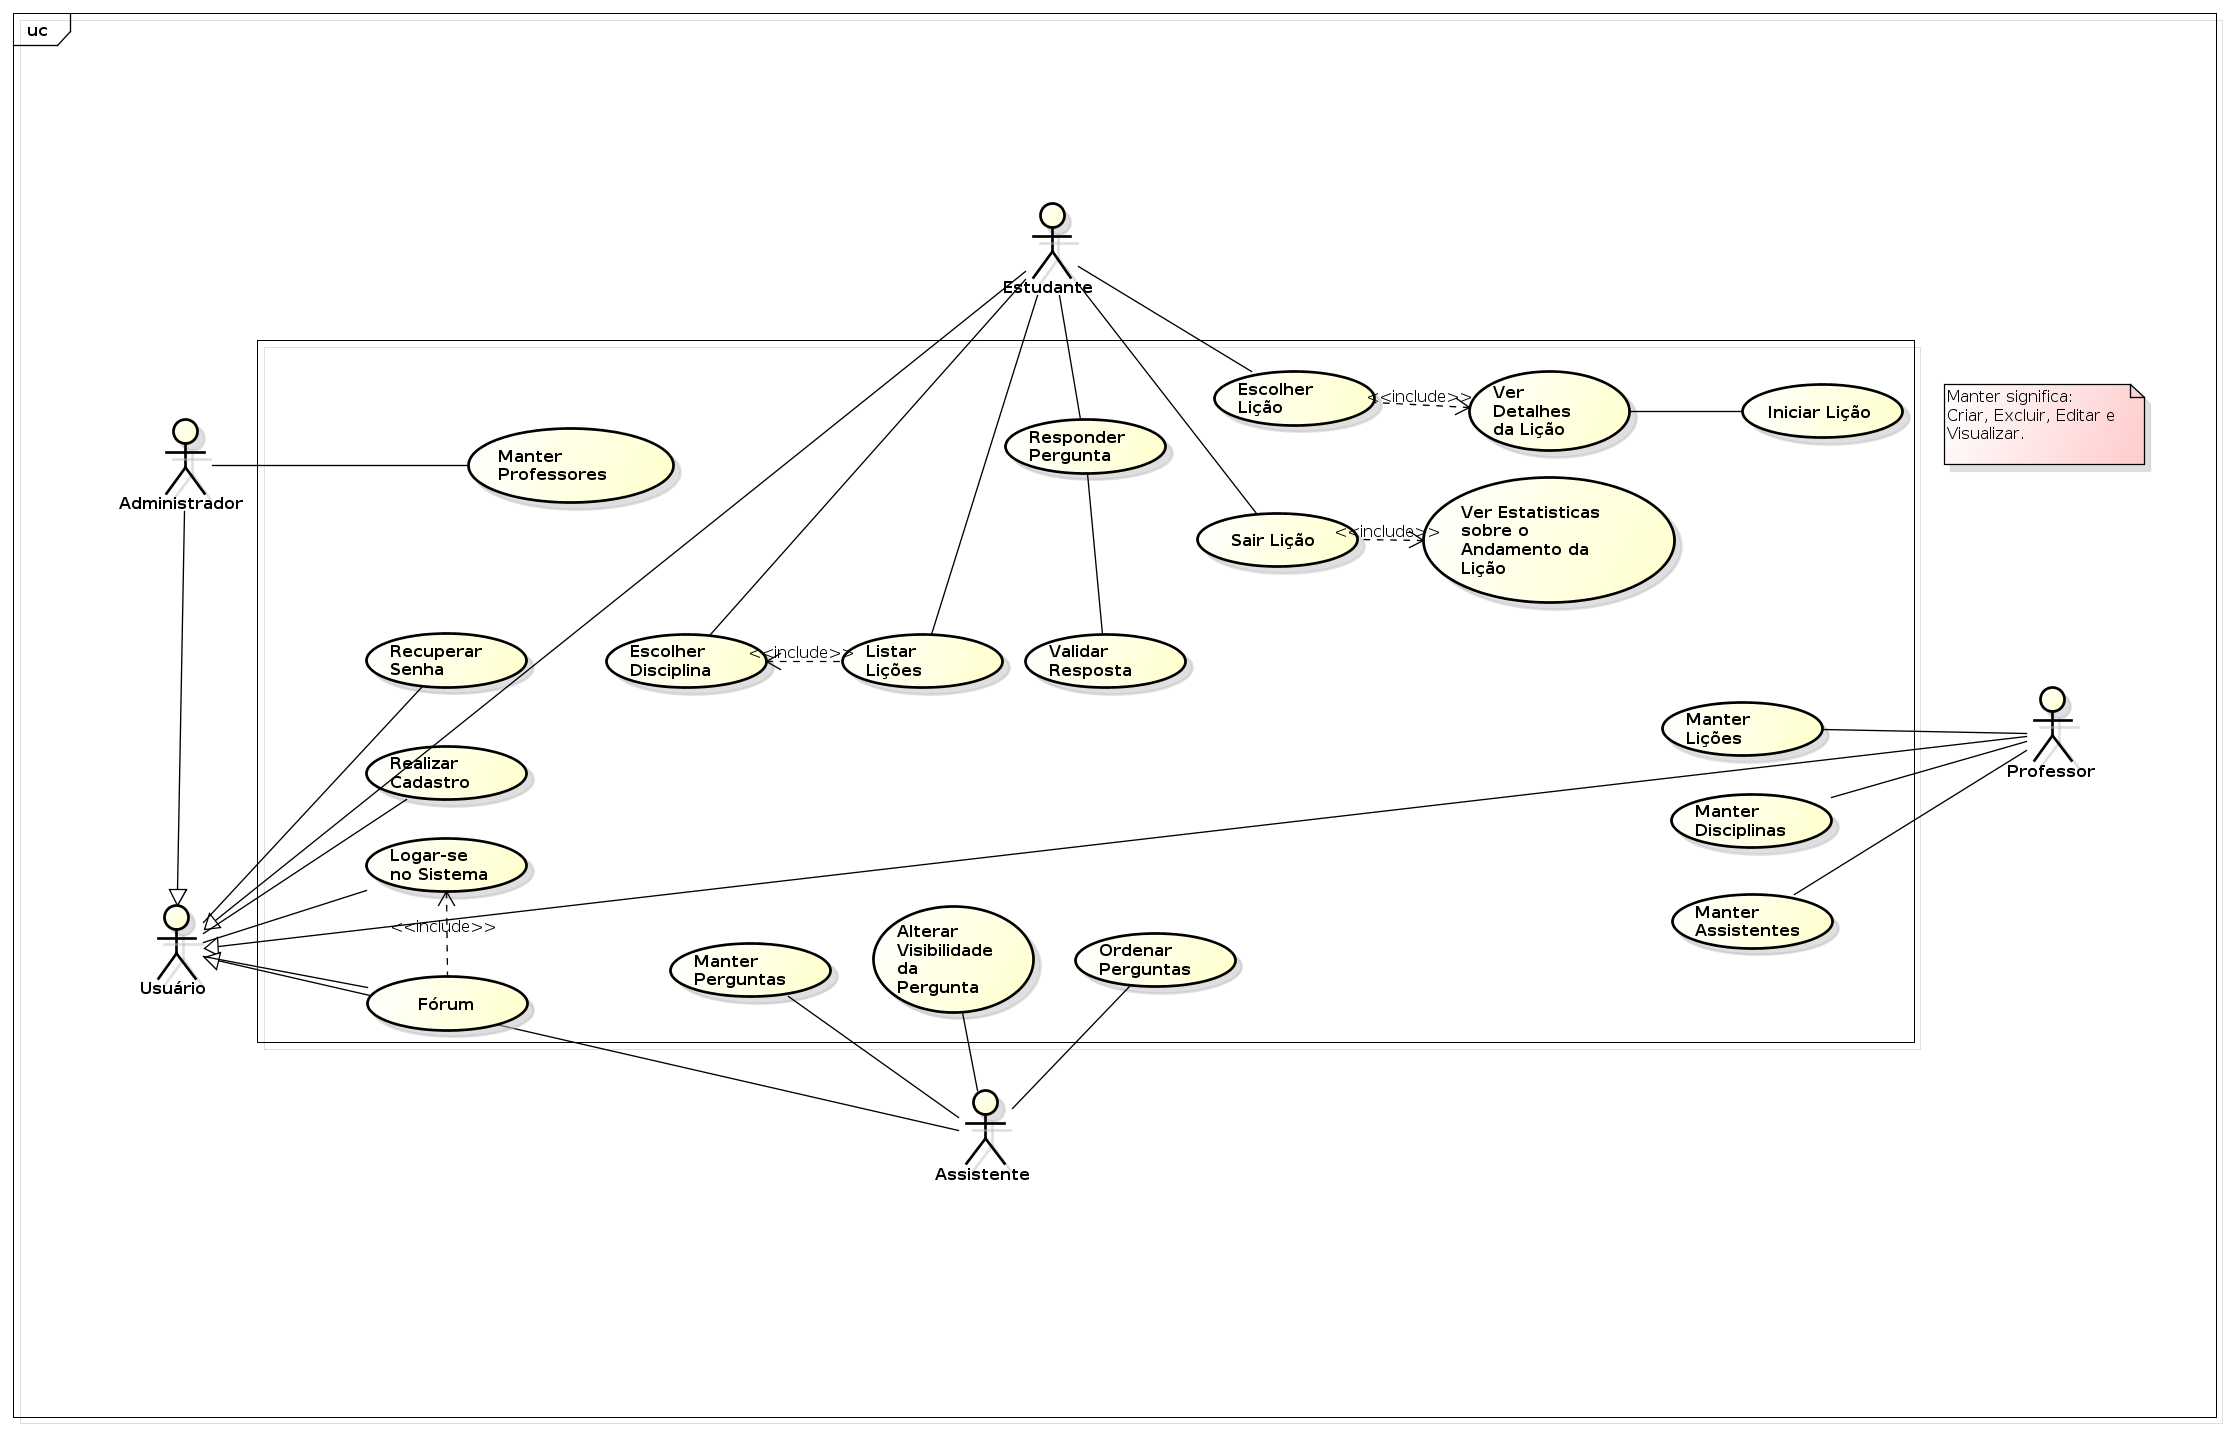
\includegraphics[width=\textwidth]{figuras/figura_casos_de_uso}}
}{
  \Fonte{Elaborado pelo autor}
}	
\end{figure}

\subsection{Descri\c{c}\~ao dos Casos de Uso}

\begin{alineascomponto}
	\item Manter Professor: O Administrador terá uma opção onde poderá manter 
professores: isso funcionara da seguinte forma: Para cadastrar, o Administrador 
logado, gera um código de alguns caracteres e dar ao professor, o professor de 
posse desse código, entra na tela de cadastro dos usuário e escolhe o tipo de 
usuário que ele quer se cadastrar e informa o código de acesso que ele possui, 
assim ele terá permissão para se cadastrar como Professor.

	\item Manter Assistente: De forma análoga ao Administrador, o professor 
também irá gerar um código e entregar ao assistente, o assistente de posse 
desse código irá entrar na tela de cadastro do sistema, informar o tipo de 
usuário e o código de acesso.

	\item Recuperação de Senha: No momento do cadastro, cada usuário devera 
indicar um email v\'alido, caso futuramente o usuário necessite 
alterar a senha, um email será enviado à esse email cadastrado com um link onde 
o mesmo poder\'a acessar para recuperar a senha.

	\item Manter Conte\'udos: Apenas os professores terão permissão para manter 
conte\'udos e lições, ao adicionar uma lição, ele terá que informar apenas o 
nome da lição e ao adicionar uma lição, ele terá que informar os 
Pré-Requisitos(Outras lições que eles recomendam ter sido concluídas para se 
prosseguir na atual) e Sugestões de Estudo (outras lições que eles recomendam 
seguir após concluir essa lição) para aquela lição assim como a quantidade 
máxima de pulos que o aluno poderá realizar naquela lição.

	\item Manter Problemas: Cada lição possuirá uma lista de problemas e os 
mesmos serão adicionadas pelos assistentes. Quando um assistente adicionar 
um problema, ele terá de informar a qual lição que ele pertence, os itens que 
ela terá, assim como o item correto, a ajuda caso esse problema necessite ter, 
a quantidade de pontos que ele terá e se ele irá ficar visível imediatamente 
para os alunos ou não.

	\item Ver Detalhes da Lição: Quando o aluno optar por responder as perguntas 
de uma determinada lição, antes de mais nada, ele precisa saber os detalhes 
daquela lição, detalhes do tipo: Quantidade de questões, Máximo de Saltos 
Permitidos, Pré-Requisitos, Curiosidades sobre o conteúdo daquela lição.

	\item Sair da Lição: Enquanto o aluno estiver resolvendo os problemas, o 
sistema devera lhe oferecer a opção dele sair da lição, quando ele sair, ele 
terá de ver as estatísticas referentes ao andamento dele naquela lição como: 
Acertos, Erros, Saltos, Quantidade de Pontos Acumulados e também uma lista com 
as lições sugeridas.
	
	\item Ordenar Problemas: Quando o bolsista adicionar um problema, ela será 
adicionada automaticamente logo depois dos outros problemas daquela lição(se 
pensarmos numa lista), mas ele deverá ter uma opção onde apenas arrastando 
os problema de posição ele possa reordena-los, utilizando apenas o mouse.

\end{alineascomponto}

\addtocontents{toc}{\protect\setcounter{tocdepth}{1}}
		\apendice{\textbf{DOCUMENTO DE ARQUITETURA}}\label{ap:arquitetura}
\addtocontents{toc}{\protect\setcounter{tocdepth}{0}}

\section{Introdução}
Neste documento detalharemos a arquitetura do sistema proposto para o projeto 
AskMath. Como o projeto é voltado para a web, o sistema é formado por diversos 
padrões de projetos de mercado, principalmente, padrões orientados a objetos. 
Vamos destacar cada parte da arquitetura escolhida para a fácil compreensão de 
outras equipes que venham a trabalhar no projeto, seguindo a risca seu modelo 
para permitir que o sistema seja facilmente modificado ou incrementado sem que a 
estrutura do software seja perdida.

\section{Objetivos}
\begin{alineascomponto}
	\item Prover uma visão geral da arquitetura do projeto, detalhando cada 
parte da estrutura do sistema para permitir a compreensão do mesmo.
    \item Permitir que este documento seja utilizado por outras equipes de 
desenvolvimento que dar\~ao continuidade ao projeto, quanto a novos 
integrantes inseridos na equipe.
    \item Apresentar aos \textit{stakeholders} uma visão de alto nível de como o 
sistema é implementado e como est\'a estruturado.
    \item Aumentar o desempenho e a robustez, bem como a capacidade de 
distribuição e manutenibilidade do sistema.
\end{alineascomponto}

\section{Considerações Gerais}
As definições de arquitetura do processo de desenvolvimento do software esta 
preocupado como o sistema deve ser organizado e com a estrutura geral do 
sistema, estas definições tem que atender as especificações do projeto, desde as 
especificações de segurança, regras de negócio, até a parte de persistência de 
banco de dados. As decisões de projeto de arquitetura têm efeitos profundos 
sobre a possibilidade de o sistema atender ou não aos requisitos críticos, como 
desempenho, confiabilidade e manutenibilidade.

As definições da arquitetura atendem as especificações de projeto documentadas 
até o presente momento, apresentando um modelo completo do sistema que mostre 
seus diferentes componentes, suas interfaces e conexões.

\section{Responsabilidades}
Toda a equipe de desenvolvimento é responsável por elaborar este documento  e 
por manter a integridade do mesmo durante o processo de desenvolvimento. Cada 
membro deve:
\begin{alineascomponto}
	\item Analisar todas as mudanças arquiteturais significativas e 
documentá-las;
    \item Ao verificar uma possível alteração na arquitetura, convocar uma 
reunião com toda e equipe para discutir a possível alteração. 
\end{alineascomponto}

\section{Arquitetura}
A arquitetura foi desenvolvida para ser de baixo acoplamento e que ao mesmo 
tempo fosse independente de tecnologias existentes do mercado, sendo assim, 
poderíamos por exemplo futuramente trocar o framework Django pelo o Spring, e o 
mesmo seria transparente para os programadores e para o sistema.

\subsection{Elementos que compõe a Arquitetura}
A arquitetura é composta por elementos, em que em conjunto produzem o produto 
final. Esses elementos são: Database, Models, Views e Templates.

Nos tópicos a seguir, descreveremos cada um dos componentes e o seu papel  dentro 
da arquitetura como um todo, além de discutirmos as tecnologias e os padrões 
adotados para a implementação dos mesmos.

\subsubsection{Database}
No desenvolvimento de sistemas, necessitamos muitas vezes salvar as informações 
geradas para eventuais utilizações futuras das mesmas, para isso, temos disponíveis os 
banco de dados. Em geral, as linguagens de programação nos proporcionam formas 
de acessar esses dados, porém de forma muito  complexa que acaba ocasionando um 
alto acoplamento para termos de alta coesão. O framework que utilizaremos (Django), nós 
proporcionar\'a uma camada apenas de banco de dados ou camada de persistência. Nessa camada estar\~ao as entidades do sistema, que implementam funcionalidades de conexão e outros controles que são 
iguais a todos os tipos de acessos a bancos de dados. 

Com esse tipo de acesso aos dados, conseguiremos trocar facilmente de banco de 
dados sem afetar a implementação do sistema. Por exemplo, caso estejamos 
utilizando um SGBD relacional como o postgresql para armazenar os dados e 
necessitarmos migrar para um SGBD não “relacional”, os famosos banco de dados 
NoSQL, como o MongoDB, não será necessário alterar nenhum aspecto da 
implementação, pois as regras de negócio vão está totalmente separadas das 
funcionalidades de acesso ao banco de dados.

\subsubsection{Models}
São as entidades do sistema. Entidades são abstrações do mundo real modelados em 
forma de tabelas que guardarão informações no banco de dados. Nessa arquitetura, 
os modelos contemplarão também as associações entre as entidades, sendo que cada 
entidade também terá al\'em de seus atributos, um conjunto de métodos para se 
relacionar com o sistema.

Os modelos implementarão um ORM(Object-Relational Mapping) para as views 
acessarem o banco de dados, tornando o sistema independente do acesso ao banco. 

\subsubsection{Views}
Todo sistema é formado por um conjunto de regras de negócio. Uma regra de 
neg\'ocio é um fluxo lógico que deve ser processado para que seja gerado um resultado 
válido.

Uma View é responsável pela execução de um ou mais fluxos de execução que são 
modelados em um caso de uso, ou seja, uma view é uma implementação da regra de 
neg\'ocio, elas são basicamente funções que aceitam como primeiro parâmetro uma 
\textit{request} que representa uma requisição Web (além de outros parâmetros) 
vinda do usuário pelo \textit{browser}, ela irá tratar essa requisição e 
retornar uma resposta ao usuário.

Dessa forma, cada caso de uso acaba tornando se uma view, sendo que views podem 
dispor de outras views para realizarem suas tarefas. 

\subsection{Desenho geral da arquitetura}

\begin{figure}[h!]
	\centering
	\Caption{\label{fig:arquitetura} Desenho Geral da Arquitetura}	
	\UFCfig{}{
		\fbox{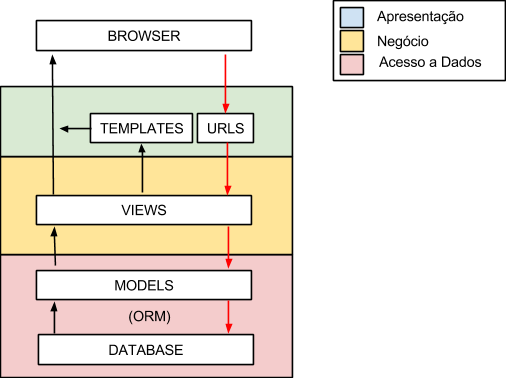
\includegraphics[width=7cm]{figuras/figura_arquitetura.png}}
	}{
		\Fonte{Elaborada pelo autor.}
	}	
\end{figure}


Nessa arquitetura, o browser do cliente utilizar\'a de uma URL para realizar uma 
requisição \`a uma view. Essa view poder\'a utilizar os models para extrair dados do 
banco de dados e ela própria criar um template e retornar como uma forma 
de resposta ao usuário, ou então, utilizar um template pronto e apenas 
moldar esses dados dentro dele e retornar isso ao browser. 

\section{Padrões de projeto}
Um padrão de projeto representa o trabalho de uma pessoa que encontrou o mesmo 
problema, tentou muitas soluções possíveis, selecionou e descreveu uma das 
melhores e você deve se aproveitar disso.

O conhecimento de padrões permite decidir o que deve ser feito e o que deve ser 
evitado. Sistemas baseados em padrões têm mais qualidade. Para o AskMath, foram analisados alguns padrões  de projeto e selecionados aqueles que poderiam ser satisfatoriamente aplicados. Nas 
se\c{c}\~oes a seguir, descreveremos cada um deles.

\subsection{Proxy}
Fornecer um substituto ou marcador da localização de outro objeto para controlar 
o acesso a esse objeto, podemos controlar o acesso aos métodos de uma entidade 
da seguinte forma: cria se uma classe EntidadeProxy que extende de Entidade, e 
reimplementa cada um dos métodos, nessa nova implementação, você solicitar que o 
usuário informe uma autenticação que possua acesso, ao informar, esse método ira 
apenas chamar o método da Entidade.   

\subsection{Chain of Responsibility}
Evitar o acoplamento do remetente de uma solicitação ao seu receptor, ao dar a 
mais de um objeto a oportunidade de tratar a solicitação. Encadear os objetos 
receptores, passando a solicitação ao longo da cadeia até que um objeto a trate.

\section{Objetivos e Restrições Arquiteturas}

Apresentaremos aqui os requisitos e objetivos do software que têm algum impacto 
na arquitetura, tais como: segurança, proteção de dados, privacidade, 
portabilidade, distribuição, reuso. Também são descritos nesta seção restrições 
arquiteturais que se aplicam ao projeto, tais  como:  estratégias  de  modelagem e implementação, ferramentas de  desenvolvimento, sistemas legados. 

\subsection{Requisitos básicos}
\begin{alineascomponto}
	\item Ubuntu Server como sistema operacional de produção.
	\item Utilização apenas de componentes \textit{open source}.
	\item PostgreSQL como sistema de gerenciamento de banco de dados.
	\item Django como framework de desenvolvimento.	
	\item O sistema devera ser Web.
\end{alineascomponto}

\subsection{Estratégias de implementação}
\begin{alineascomponto}
	\item Persistência de tipagem (ex: formato de CPF, Data) devem ser feitos 
tanto no cliente através de Javascript, como no servidor através de 
regex(Regular Expression).
	\item Persistência de obrigatoriedade, verificar se todos os campos 
obrigatórios foram  preenchidos deve ser feito tanto no cliente via javascript 
como no servidor e nas duas opções deve-se apresentar alertas caso algum campo 
seja enviado vazio para a requisição.
    
\end{alineascomponto}

\addtocontents{toc}{\protect\setcounter{tocdepth}{1}}
		\apendice{\textbf{QUESTIONÁRIO INICIAL}}\label{ap:questionario_inicial}
\addtocontents{toc}{\protect\setcounter{tocdepth}{0}}

\noindent \textbf{Pesquisa:} Questionário Inicial

\noindent
Código: 

\section{Sobre}

Este questionário faz parte de um trabalho de dissertação de Bacharelado em Sistemas de Informação e tem como objetivo recolher dados sobre sua relação com as disciplinas de Matemática e com o uso do computador nas aulas e também fora delas.

Na publicação dos resultados desta pesquisa, sua identidade será mantida no mais rigoroso sigilo. Serão omitidas todas as informações que permitam identificá-lo(a). 

\section{Dados Biográficos}

\begin{enumerate}
	\item Idade: 
    \item Género: $\ocircle$ Masculino $\ocircle$ Feminino
\end{enumerate}

\section{Relação com a Matemática}

\begin{enumerate}
\item Quanto tempo, por semana, você se dedica estudando Matemática? \\
$\ocircle$ Menos de 1 hora $\ocircle$ 1 a 3 horas $\ocircle$ 3 a 5 horas $\ocircle$ Mais de 5 horas

\item O que você pensa sobre a Matemática? \\
$\ocircle$ Muito Díficil $\ocircle$ Díficil $\ocircle$ Aceitável $\ocircle$ Fácil $\ocircle$ Muito Fácil

\item Você gosta de estudar matemática? Por quê? \\
$\ocircle$ Sim $\ocircle$ Não $\ocircle$ Um Pouco \\
\noindent\rule{\textwidth}{0.4pt}
\noindent\rule{\textwidth}{0.4pt}

\item Em sua opinião, qual é a melhor maneira de aprender matemática? \\
$\ocircle$ Por meio da explicação do professor $\ocircle$ Por meio de exercícios individuais \\
$\ocircle$ Por meio de exercícios em grupos \\
Outra maneira: \\
\noindent\rule{\textwidth}{0.4pt}

\end{enumerate}

\section{Uso do Computador Fora da Aula}
\begin{enumerate}
\item Você tem computador? \\
$\ocircle$ Sim $\ocircle$ Não 
    
\item Voc\^e possui computador com acesso a internet fora da universidade? \\
$\ocircle$ Sim $\ocircle$ Não
    
\item Você gosta de usar computadores? \\
$\ocircle$ Gosto Muito $\ocircle$ Gosto $\ocircle$ Gosto Pouco $\ocircle$ Não Gosto

\item Durante o semestre letivo, com que objetivo e frequência você usa o computador para: \\
\begin{tabular}{lllll}
	Fazer trabalhos acadêmicos: & $\ocircle$ Nunca & $\ocircle$ Raramente & $\ocircle$ Às Vezes & $\ocircle$ Sempre \\
	Pesquisar na internet: & $\ocircle$ Nunca & $\ocircle$ Raramente & $\ocircle$ Às Vezes & $\ocircle$ Sempre \\
	Comunicar-se com amigos: & $\ocircle$ Nunca & $\ocircle$ Raramente & $\ocircle$ Às Vezes & $\ocircle$ Sempre \\
	Usar sites educativos: & $\ocircle$ Nunca & $\ocircle$ Raramente & $\ocircle$ Às Vezes & $\ocircle$ Sempre \\
	Outra(s): \\
	\multicolumn{5}{l}{\noindent\rule{\textwidth}{0.4pt}} \\
	\multicolumn{5}{l}{\noindent\rule{\textwidth}{0.4pt}} \\
\end{tabular}

\item Com que frequência você utiliza sites educativos? \\
\begin{tabular}{lllll}
	Em casa: & $\ocircle$ Nunca & $\ocircle$ Raramente & $\ocircle$ Às Vezes & $\ocircle$ Sempre \\
	Na casa de amigos: & $\ocircle$ Nunca & $\ocircle$ Raramente & $\ocircle$ Às Vezes & $\ocircle$ Sempre \\
	Em locais públicos: & $\ocircle$ Nunca & $\ocircle$ Raramente & $\ocircle$ Às Vezes & $\ocircle$ Sempre \\
	Na escola: & $\ocircle$ Nunca & $\ocircle$ Raramente & $\ocircle$ Às Vezes & $\ocircle$ Sempre \\
	Em outro(s) local(ais), qual(is)? \\
	\multicolumn{5}{l}{\noindent\rule{\textwidth}{0.4pt}} \\
	\multicolumn{5}{l}{\noindent\rule{\textwidth}{0.4pt}} \\
\end{tabular}

\item Que tipo de sites educativos você costuma usar e com qual frequência? \\
\begin{tabular}{lllll}
	Sites Informativos: & $\ocircle$ Nunca & $\ocircle$ Raramente & $\ocircle$ Às Vezes & $\ocircle$ Sempre \\
	Sites de Jogos Pedagogicos: & $\ocircle$ Nunca & $\ocircle$ Raramente & $\ocircle$ Às Vezes & $\ocircle$ Sempre \\
	Blogues: & $\ocircle$ Nunca & $\ocircle$ Raramente & $\ocircle$ Às Vezes & $\ocircle$ Sempre \\
	Outro(s), quail(s)?: \\
	\multicolumn{5}{l}{\noindent\rule{\textwidth}{0.4pt}} \\
	\multicolumn{5}{l}{\noindent\rule{\textwidth}{0.4pt}} \\
\end{tabular}

\item Com que frequencia você costuma usar sites educativos para: \\
\begin{tabular}{lllll}
	Estudar: & $\ocircle$ Nunca & $\ocircle$ Raramente & $\ocircle$ Às Vezes & $\ocircle$ Sempre \\
	Tirar dúvidas: & $\ocircle$ Nunca & $\ocircle$ Raramente & $\ocircle$ Às Vezes & $\ocircle$ Sempre \\
	Curiosidade: & $\ocircle$ Nunca & $\ocircle$ Raramente & $\ocircle$ Às Vezes & $\ocircle$ Sempre \\
	Outro(s), quail(s)?: \\
	\multicolumn{5}{l}{\noindent\rule{\textwidth}{0.4pt}} \\
	\multicolumn{5}{l}{\noindent\rule{\textwidth}{0.4pt}} \\
\end{tabular}

\end{enumerate}

\section{Uso do Computador nas Aulas}
\begin{enumerate}
\item Com que frequencia você costuma utilizar o computador na sala de aula? \\
$\ocircle$ Nunca  $\ocircle$ Raramente  $\ocircle$ Às Vezes  $\ocircle$ Sempre \\

\item Você gosta de usar computador nas aulas? \\
$\ocircle$ Gosto Muito $\ocircle$ Gosto $\ocircle$ Gosto Pouco $\ocircle$ Não Gosto

\item Para que fins você utiliza computador nas aulas? \\
\begin{tabular}{lllll}
	Realizar as tarefas: & $\ocircle$ Nunca & $\ocircle$ Raramente & $\ocircle$ Às Vezes & $\ocircle$ Sempre \\
	Estudar: & $\ocircle$ Nunca & $\ocircle$ Raramente & $\ocircle$ Às Vezes & $\ocircle$ Sempre \\
	Acessar sites educativos: & $\ocircle$ Nunca & $\ocircle$ Raramente & $\ocircle$ Às Vezes & $\ocircle$ Sempre \\
	Outro(s), quail(s)?: \\
	\multicolumn{5}{l}{\noindent\rule{\textwidth}{0.4pt}} \\
	\multicolumn{5}{l}{\noindent\rule{\textwidth}{0.4pt}} \\
\end{tabular}

\end{enumerate}

\addtocontents{toc}{\protect\setcounter{tocdepth}{1}}
		\apendice{\textbf{QUESTIONÁRIO FINAL}}\label{ap:questionario_final}
\addtocontents{toc}{\protect\setcounter{tocdepth}{0}}

\noindent \textbf{Pesquisa:} Questionário Final


\noindent
Código: 

\section{Sobre}

Este questionário faz parte de um trabalho de dissertação de Bacharelado em Sistemas de Informação e tem como objetivo 
recolher dados e opiniões sobre a utilização que fazes do Ambiente Virtual de Aprendizagem (AVA) Askmath, assim como da tua opinião relativamente à utilização do AVA e das 
tecnologias nele integradas na aprendizagem da Matemática.

Na publicação dos resultados desta pesquisa, sua identidade será mantida no mais rigoroso sigilo. Serão omitidas todas as informações que permitam identificá-lo(a). 

\section{Utilização}

\begin{enumerate}

\item Com que frequência você utilizou o AVA? \\
\begin{tabular}{lllll}
	Em casa: & $\ocircle$ Nunca & $\ocircle$ Raramente & $\ocircle$ Às Vezes & $\ocircle$ Sempre \\
	Na casa de amigos: & $\ocircle$ Nunca & $\ocircle$ Raramente & $\ocircle$ Às Vezes & $\ocircle$ Sempre \\
	Em locais públicos: & $\ocircle$ Nunca & $\ocircle$ Raramente & $\ocircle$ Às Vezes & $\ocircle$ Sempre \\
	Na escola: & $\ocircle$ Nunca & $\ocircle$ Raramente & $\ocircle$ Às Vezes & $\ocircle$ Sempre \\
	Em outro(s) local(ais), qual(is)? \\
	\multicolumn{5}{l}{\noindent\rule{\textwidth}{0.4pt}} \\
	\multicolumn{5}{l}{\noindent\rule{\textwidth}{0.4pt}} \\
\end{tabular}

\item Durante a utilização do AVA, que problema foram encontrados? \\
\begin{tabular}{lllll}
	Falta de tempo: & $\ocircle$ Nunca & $\ocircle$ Raramente & $\ocircle$ Às Vezes & $\ocircle$ Sempre \\
	Conexão com a internet: & $\ocircle$ Nunca & $\ocircle$ Raramente & $\ocircle$ Às Vezes & $\ocircle$ Sempre \\
	Lentidão no acesso a plataforma: & $\ocircle$ Nunca & $\ocircle$ Raramente & $\ocircle$ Às Vezes & $\ocircle$ Sempre \\
	Erros na plataforma: & $\ocircle$ Nunca & $\ocircle$ Raramente & $\ocircle$ Às Vezes & $\ocircle$ Sempre \\
	Outro(s), qual(is)? \\
	\multicolumn{5}{l}{\noindent\rule{\textwidth}{0.4pt}} \\
	\multicolumn{5}{l}{\noindent\rule{\textwidth}{0.4pt}} \\
	\multicolumn{5}{l}{\noindent\rule{\textwidth}{0.4pt}} \\
\end{tabular}

\item Como você avalia o AVA em relação a sua utilização como motivador para desenvolver e construir os conhecidos adquiridos nos conteúdos aprendidos? \\ 
$\ocircle$ Muito fraco  $\ocircle$ Fraco $\ocircle$ Razoável $\ocircle$ Bom $\ocircle$ Muito Bom
 
\item Como você avalia o AVA em relação a sua importância para o compartilhamento de informações e construção do conhecimento compartilhado? \\ 
$\ocircle$ Muito fraco  $\ocircle$ Fraco $\ocircle$ Razoável $\ocircle$ Bom $\ocircle$ Muito Bom

\item O quão importante você considera o AVA para auxiliar no processo de aprendizagem? \\ 
$\ocircle$ Nada importante  $\ocircle$ Pouco Importante $\ocircle$ Razoável $\ocircle$ Importante $\ocircle$ Muito Importante

\end{enumerate}

\section{Comunicação}

\begin{enumerate}
  \item Como você avalia as ferramentas de comunicação do AVA em seu uso para promover uma maior interação entre os alunos? \\
  $\ocircle$ Muito fracas  $\ocircle$ Fracas $\ocircle$ Razoável $\ocircle$ Boas $\ocircle$ Muito Boas

  \item Como você avalia a utilização do AVA para promover uma maior interação com os conteúdos? \\
  $\ocircle$ Muito fraco  $\ocircle$ Fraco $\ocircle$ Razoável $\ocircle$ Bom $\ocircle$ Muito Bom

\end{enumerate}

\section{O Ambiente Virtual de Aprendizagem}

\noindent
Como você avalia o AVA para as seguintes afirmações:\\

\noindent
\resizebox{\textwidth}{!}{
\begin{tabular}{|p{8cm}|p{1.8cm}|c|c|c|p{2cm}|}
	\hline
	O ambiente virtual de aprendizagem Matemática como complemento ao ensino presencial: & Discordo  totalmente & Discordo & N\~ao sei & Concordo & Concordo totalmente \\
	\hline
	Proporcionou um maior acompanhamento pelo professor & $\ocircle$ & $\ocircle$ & $\ocircle$ & $\ocircle$ & $\ocircle$ \\
	\hline
	Apoiou seus estudos de forma a superar suas dificuldades & $\ocircle$ & $\ocircle$ & $\ocircle$ & $\ocircle$ & $\ocircle$ \\
	\hline
	Permitiu você adquirir novos conhecimentos & $\ocircle$ & $\ocircle$ & $\ocircle$ & $\ocircle$ & $\ocircle$ \\
	\hline
	Proporcionou um maior acompanhamento pelo professor & $\ocircle$ & $\ocircle$ & $\ocircle$ & $\ocircle$ & $\ocircle$ \\
	\hline
	Contribuiu para aumentar meu interesse em relação a Matemática & $\ocircle$ & $\ocircle$ & $\ocircle$ & $\ocircle$ & $\ocircle$ \\
	\hline
	Ajudou na aprendizagem dos conteúdos da disciplina & $\ocircle$ & $\ocircle$ & $\ocircle$ & $\ocircle$ & $\ocircle$ \\
	\hline
	Melhorou meus resultados nas disciplinas & $\ocircle$ & $\ocircle$ & $\ocircle$ & $\ocircle$ & $\ocircle$ \\
	\hline
	Facilitou o compartilhamento de opiniões & $\ocircle$ & $\ocircle$ & $\ocircle$ & $\ocircle$ & $\ocircle$ \\
	\hline
	Permitiu uma aprendizagem mais autônoma e responsável & $\ocircle$ & $\ocircle$ & $\ocircle$ & $\ocircle$ & $\ocircle$ \\
	\hline
	Permitiu uma aprendizagem mais desafiante, permitindo um maior controle sob ela & $\ocircle$ & $\ocircle$ & $\ocircle$ & $\ocircle$ & $\ocircle$ \\
	\hline
	Permitiu a troca de ideias entre os alunos & $\ocircle$ & $\ocircle$ & $\ocircle$ & $\ocircle$ & $\ocircle$ \\
	\hline
\end{tabular}
}

\section{Sugestões}
Espaço destinado a comentários, sugestões e críticas. Diga o que você mudaria no Askmath:\\
\noindent\rule{\textwidth}{0.4pt}
\noindent\rule{\textwidth}{0.4pt}
\noindent\rule{\textwidth}{0.4pt}
\noindent\rule{\textwidth}{0.4pt}

\addtocontents{toc}{\protect\setcounter{tocdepth}{1}}
	\imprimiranexos
		% Adicione aqui os anexos do seu trabalho
		\anexo{Exemplo de Anexo}
\label{an:exemplo-de-anexo}

Texto texto texto texto texto texto texto  texto texto texto  texto texto texto  texto texto texto  texto texto texto  texto texto texto  texto texto texto  texto texto texto  texto texto texto  texto texto texto  texto texto texto. 
	\imprimirindice

\end{document}